\chapter{Using Fourier transform phase for the measurement of radial velocity}
\label{\thechapter}
\label{ch:Methods}
\addcontentsline{lof}{chapter}{\protect\numberline{\arabic{chapter}} {\nameref{\thechapter}}}

%----------------------------------------------------------------------------------------

\rule{\textwidth}{1.6pt}
\minitoc
\clearpage

%----------------------------------------------------------------------------------------

%{\em CGT: This needs a bit more helpful an introduction. That is WHY the fourier trasform is being explored as
%a way to measure radial velocity. and specifically, so that you can try to tell the difference between bulk line shifts, and line profile deformations.
%I think the folloing does a slightly better job of that.}

This chapter introduces a new method for measuring radial velocities. Specifically, it uses the Fourier transform
of a line profile (or cross-correlation profile) to try and distinguish between the effects of a bulk shift in that profile
(i.e. a radial velocity shift of the profile), opposed to a change in the line profile shape which can produce an
apparent radial velocity shift. We examine the impact on the Fourier transformed components of a line profile of both bulk line shifts, and line profile deformations, with the aim of developing tools to distinguish between these two cases.

%%----------------------------------------------------------------------------------------	
%\pagebreak
%%----------------------------------------------------------------------------------------	

\section{Phase analysis of Fourier transform for the measurement of line shift}
\label{\thesection}
\label{ch:FT_line_shift}


\subsection{Translation property of Fourier transform}

The translation of a function (in our case a spectral line profile) can be examined in both its original real
space, and in its Fourier transformed space. Because Fourier techniques are often used to handle time domain data,
this shift in real space can be variously considered described as either time shifting or translation. In this chapter 
we will use ``time shifting'', ``translation'' and ``velocity shifting'' interchangeably to refer to a shift of a function
in real space. We will refer to Fourier transformed functions as being in the ``frequency domain'' regardless of whether they have actual dimensions of 1/time, 1/length or 1/velocity.

Let us consider a function $h(x)$ be a signal $f(x)$ delayed (or shifted) by an amount $x_0$:
\begin{equation}
	h(x) = f(x-x_0).
\label{eq:FT1}
\end{equation}
In the frequency domain, we will then have 
\begin{equation}
	\hat{h}(\xi) = e^{-2 \pi ix_0 \xi} \hat{f}(\xi),
\label{eq:FT2}
\end{equation}
where the circumflex denotes the Fourier transform of a function. $\hat{h}(\xi)$ and $\hat{f}(\xi)$ 
will therefore differ by a frequency dependent phase angle: 
\begin{equation}
	\Delta \phi(\xi) = -2 \pi x_0 \xi,
\label{eq:PhaseShift}
\end{equation}
while the power spectral density will remain unchanged (as $\mid e^{-2 \pi ix_0 \xi}\mid ^2 = 1$).


\subsection{Intuitive explanation}

The translation property of the Fourier transform follows mathematically from the nature of the transform. 
A (perhaps) more intuitive way to see this is that since the Fourier transform is defined 
\begin{equation}
	\hat{f}(\xi) = \int_{-\infty}^{\infty} f(x) e^{-2 \pi ix \xi} dx, 
\label{eq:FT3}
\end{equation}
it decomposes the function $f(x)$ into a frequency representation $\hat{f}(\xi)$, such that the function $f(x)$ is expressed  
as the sum of \textit{all} the orthogonal basis $e^{2 \pi ix \xi}$ times a set of their components $\hat{f}(\xi)$ (i.e.
by the inverse Fourier transform):
\begin{equation}
	f(x) = \int_{-\infty}^{\infty} \hat{f}(\xi) e^{2 \pi ix \xi} d\xi. 
\end{equation}

This means that shifting $f(x)$ by $x_0$ is equivalent to shifting \textit{all} the orthogonal basis functions by $x_0$, which becomes $e^{2 \pi i(x-x_0) \xi} = e^{2 \pi i x \xi} \cdot e^{-2 \pi ix_0 \xi}$. This is how the $e^{-2 \pi ix_0 \xi}$ term in Eq.~\ref{eq:FT2} arises -- it quantifies this phase difference. 
\footnote{For a simplified vision bridging a shift of the signal in the time domain and a phase difference in the frequency domain, imagine any real continuous function is a sum of sines and cosines. Changing the phase angle in the sines and cosines results in shifts in the function.}

The fact that the power spectrum density remains the same can also intuitively seen, because shifting the signal as a whole 
doesn't add or remove any frequency information. 


\subsection{Practical Use}

From Eq.~\ref{eq:PhaseShift}, we see that the phase shift $\Delta \phi(\xi)$ is proportional to the frequency $\xi$
with a constant gradient or slope 
\footnote{We use $\Delta$ to refer to the phase difference between a shifted line profile and a unshifted~/~referenced line profile, while the derivative to refer to the response of $\Delta \phi)$ to $\xi$.}
\begin{equation}
	\dv{(\Delta \phi)}{\xi} = -2 \pi x_0
\label{eq:gradient}
\end{equation}
Obtaining this (in principle) is straightforward via a simple linear regression model fit to a plot of $\Delta \phi(\xi)$ versus $\xi$ 
 (see e.g. Fig.~\ref{fig:FT}), so that
\begin{equation}
	x_0 = -\frac{1}{2 \pi}\dv{(\Delta \phi)}{\xi}
\label{eq:line_shift}
\end{equation}

%-------------
\begin{figure}[tbp]
\centering
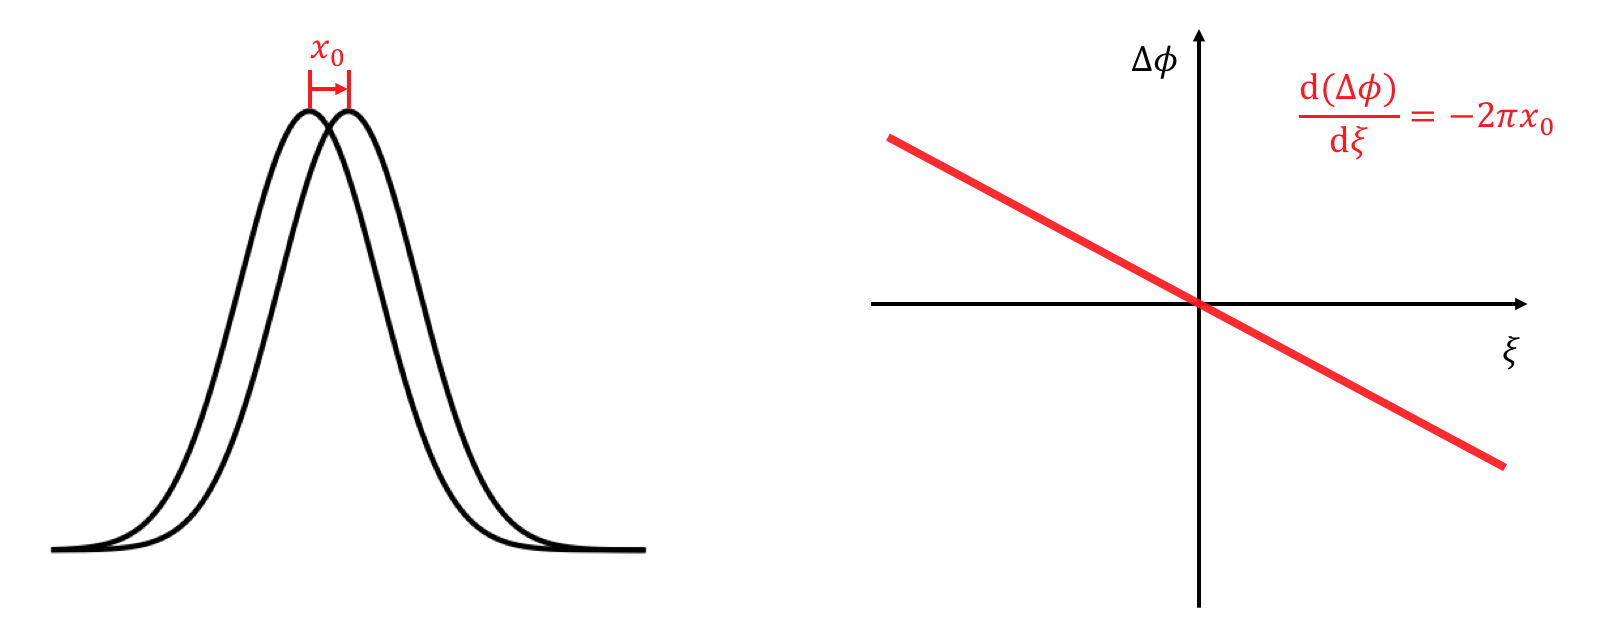
\includegraphics[width = 0.99 \linewidth]
{./Figures/Methods/FT.png}
\caption[Translation property of Fourier transform]
{The left panel shows a signal (or a spectral line profile in the following context) shifted by an amount $x_0$. 
The right panel is the differential phase spectral density diagram (i.e. differential phase spectrum). 
The model shows a perfectly linear correlation 
between $\Delta \phi(\xi)$ and $\xi$ with the constant slope $-2 \pi x_0$.}
\label{fig:FT}
\end{figure} 
%-------------

By analogy with the definition of power spectral density, we describe $\phi(\xi)$ the ``phase spectral density'' and hence $\Delta \phi(\xi)$ the ``differential phase spectral density''. 

In principle then, an  analysis of the phase shift in the frequency domain of the Fourier components of a line profile will provide a means of measuring a bulk line shift in real space. 
% More importantly,
% it may provide a means of separating  an apparent radial velocity shift into the components due to bulk line shift, 
% and line profile shape change.


%----------------------------------------------------------------------------------------	

\subsection{Initial tests}
\label{sec:Initial_tests}

We performed an initial test to determine whether we can correctly recover known shifts of a line profile  
from an analysis of the phase shift in the frequency domain of the Fourier transform of shifted line profiles.

We generated a spectral line profile based on the cross-correlation function of observed HARPS spectra
with the software SOAP 2.0 \cite{Dumusque2014SOAP}. This was replicated 100 times, with a very small amount of 
noise (equivalent to a S/N = 10,000) injected in each of the line profiles. These profiles were then
subjected to radial velocity shifts evenly spaced between 0 and 10\,m/s (Fig.~\ref{fig:line_profiles12}). 

%-------------
\begin{figure}[tbp]
    \begin{subfigure}[b]{0.49\textwidth}
        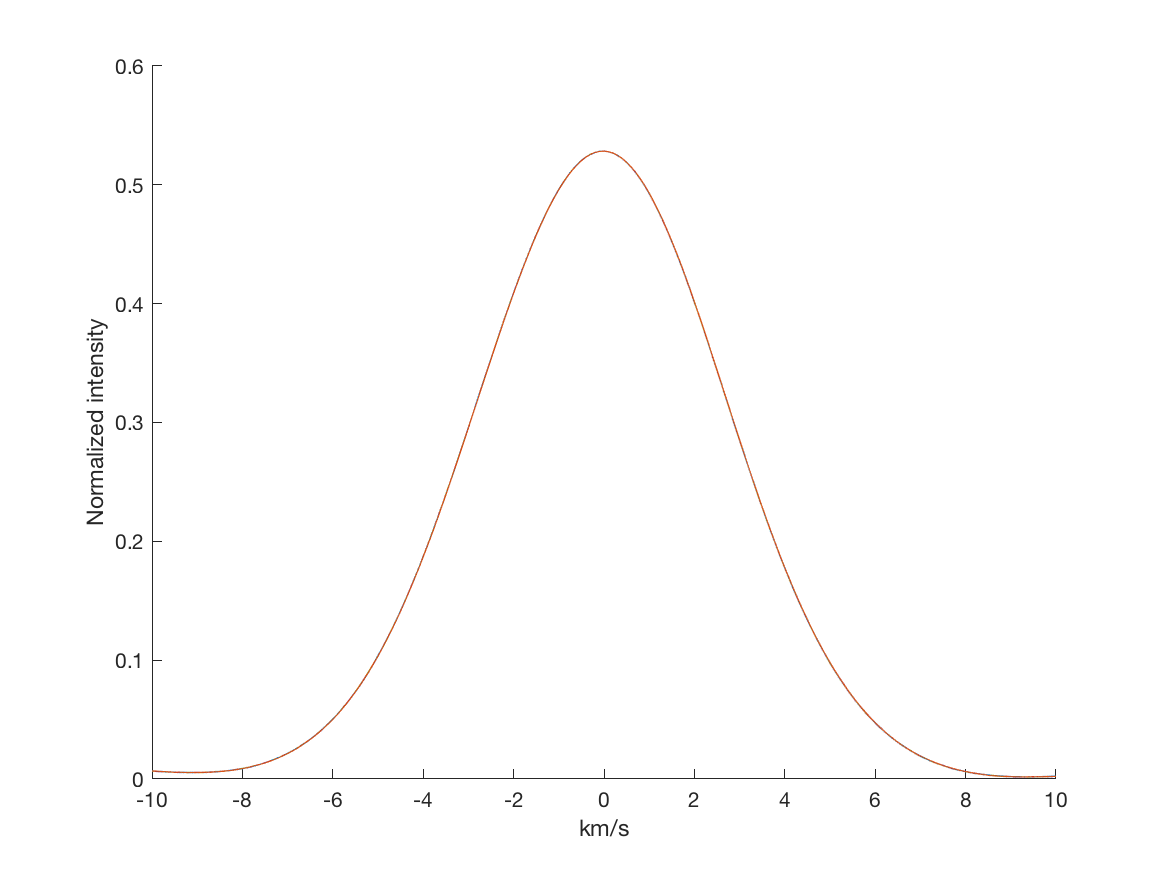
\includegraphics[width=\textwidth]{./Figures/Methods/1-Line_Profile.png}
        \caption{Line profile (stacked)}
        \label{fig:line_profiles}
    \end{subfigure}
	~
    \begin{subfigure}[b]{0.49\textwidth}
        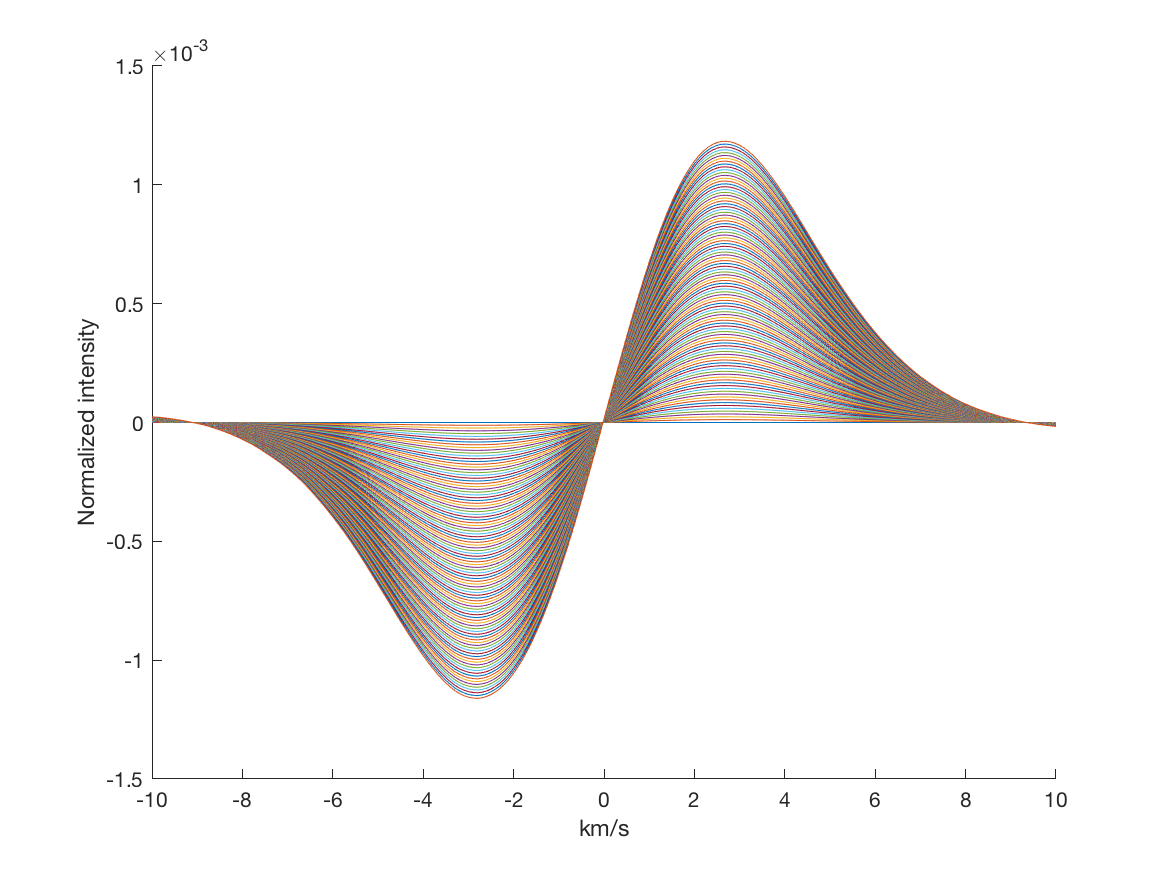
\includegraphics[width=\textwidth]{./Figures/Methods/1-Differential_line_Profile.png}
        \caption{Differential line profile}
        \label{fig:differential_line_profiles}
    \end{subfigure}	
    
    \caption[100 shifted HARPS-like line profiles]{(a) the shifted line profiles plotted on top of each other, showing that the $\pm$0-10\,m/s shifts are very small compared to the line profile width. (b) the shifted line profiles with the unshifted line profile subtracted from each. Note that for the sake of clarity, the differential line profiles are plotted noise-free and only 10 out of 100 profiles are presented.}
\label{fig:line_profiles12}
\end{figure}	
%-------------

The Fourier transform of these 100 spectral line profiles divides the information into two parts: 
(1) the power spectra (Fig.~\ref{fig:power_spectrum}) and (2) the phase spectra (shown in Fig.~\ref{fig:dps}
as the differential phase spectra relative to the phase spectrum for the unshifted line profile). 

%-------------
\begin{figure}[tbp]	
    \begin{subfigure}[b]{0.49\textwidth}
        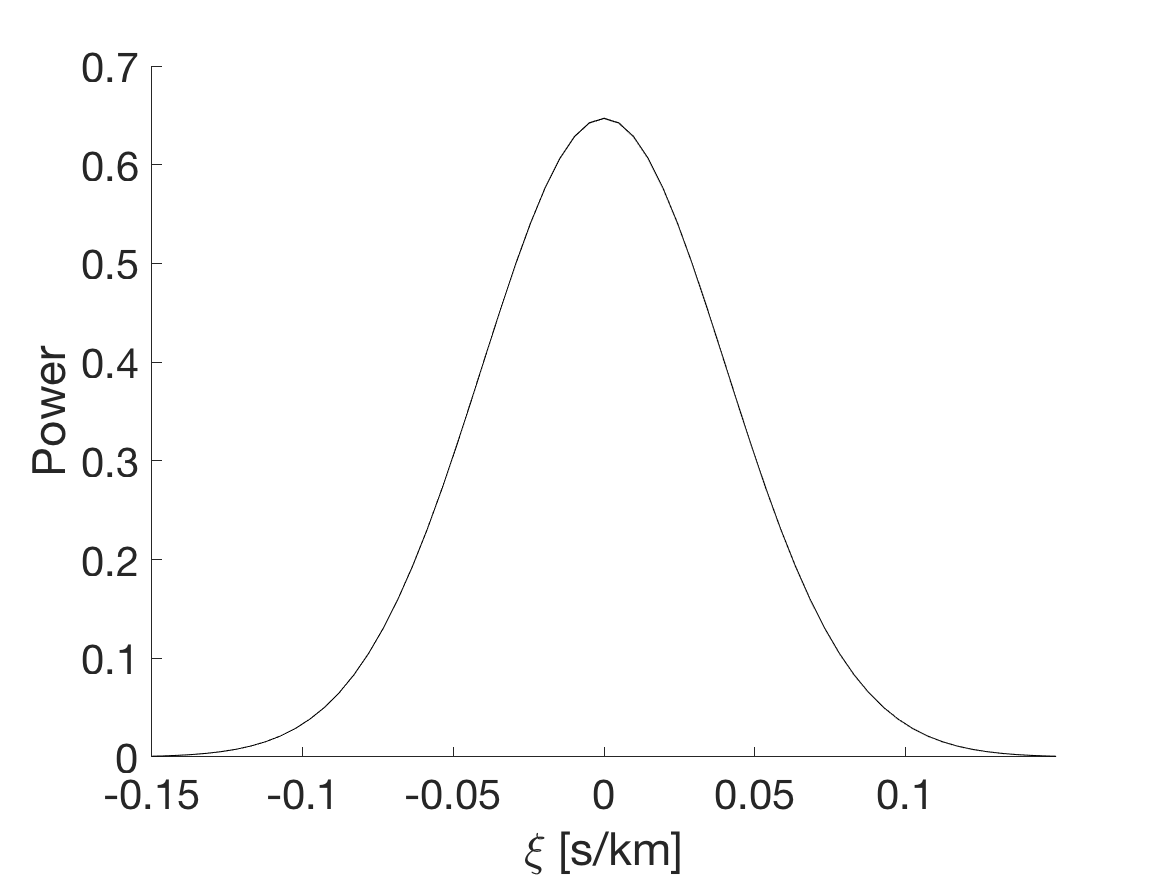
\includegraphics[width=\textwidth]{./Figures/Methods/2-FT_power.png}
        \caption{Power spectrum (stacked)}
        \label{fig:power_spectrum}
    \end{subfigure}
	~
    \begin{subfigure}[b]{0.49\textwidth}
        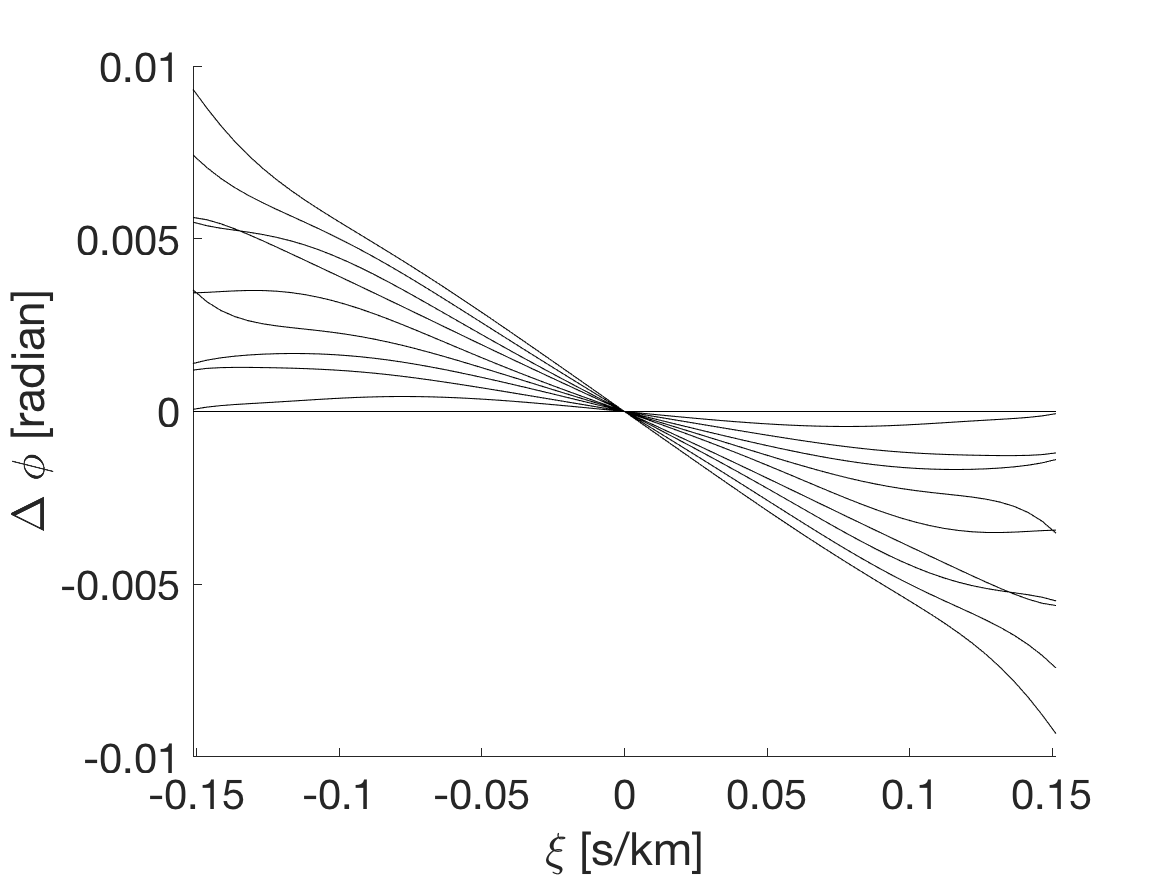
\includegraphics[width=\textwidth]{./Figures/Methods/4-Relative_phase_angle.png}
        \caption{Differential phase spectrum}
        \label{fig:dps}
    \end{subfigure}	
    \caption[Fourier transform of 100 shifted line profiles]
    {The Fourier transform of these shifted line profile divides the information in each into (a) their power spectra and (b) their phase spectra (here plotted differential compared to that of the unshifted profile). A line shift in the time domain produces an unchanged power spectrum in the frequency domain. It does, however, produce phase shift which we see as linear trends in the differential phase spectra as a function of frequency. Note that for demonstration clarity, only 10 out of 100 differential phase spectra are presented.}
\label{fig:FT_process}
\end{figure}    
%-------------

%{\em CGT: whereas the frequency ranges plotted in 2,.2a and 2.2b are the same [are they really? are you sure the axis on 2.2b should not be in m/s instead of km/s?]
%, the ranges plotted in 2.3a and 2.3b are different. You don't really say why. Until later when you make comments about "noise".
%I suggest you should make both the plots over the same range, and then *point out* the impact of noise,
%and why you have chosen to limit your fits to a smaller frequency range (and justify that choice),}

We see that most Fourier transform information is concentrated towards the centre of the power spectrum (i.e. the lower frequency range). The differential phase spectra are expected linear (as Fig.~\ref{fig:FT} demonstrated). Its deviation from linearity comes from the noise that we injected, which will be discussed later. 

The slope of each differential phase spectrum indicates the shift of each line profile relative to 
the unshifted line profile. It should be weighted by the amplitude of the power, meaning the lower frequencies 
are higher weighted. We therefore calculate the radial velocity shift for each shifted line profile
using two methods: 
\begin{enumerate}
	\item the $RV_\text{FT}$ using Eq.~\ref{eq:line_shift}, weighted by the power spectrum
	\item the $RV_\text{Gaussian}$ as traditionally measured from the line centroid by fitting a Gaussian to each line profile.
\end{enumerate}
We can then compare the results with the (known) input line shift where we see the expected strong 1:1 correlation (Fig.~\ref{fig:rv_recovery})\footnote{The line of best fit of a linear regression model presents a slope of $1.003\pm0.006$ with 95\% confidence bounds. 
% The uncertainty of the slope is derived from the uncertainty of each measured $RV_\text{FT}$, which is further derived from the uncertainty of the phase measurement, described by the magnitude of the power spectrum.
}. The root-mean-square (rms) of the residuals (or interchangeably used as standard deviation when the mean is zero) are both $\sigma_\text{FT} = \sigma_\text{Gaussian} = 0.08$ m/s, identical up to two decimal places, indicating the expected radial velocities are consistently reduced. In fact, the almost overlapping residual in Fig.~\ref{fig:rv_recovery} means that the two methods are so coherently different from the input radial velocity (by a small amount), concludes that such a deviation comes from the photon noise intrinsic to the line profile rather than the methods themselves. 

{\em CGT: How do these comare which what you'd expect from the S/N and the intrinsic line width (should say at some int what the intrinsic line width is}.

%-------------
\begin{figure}[tbp]
\centering
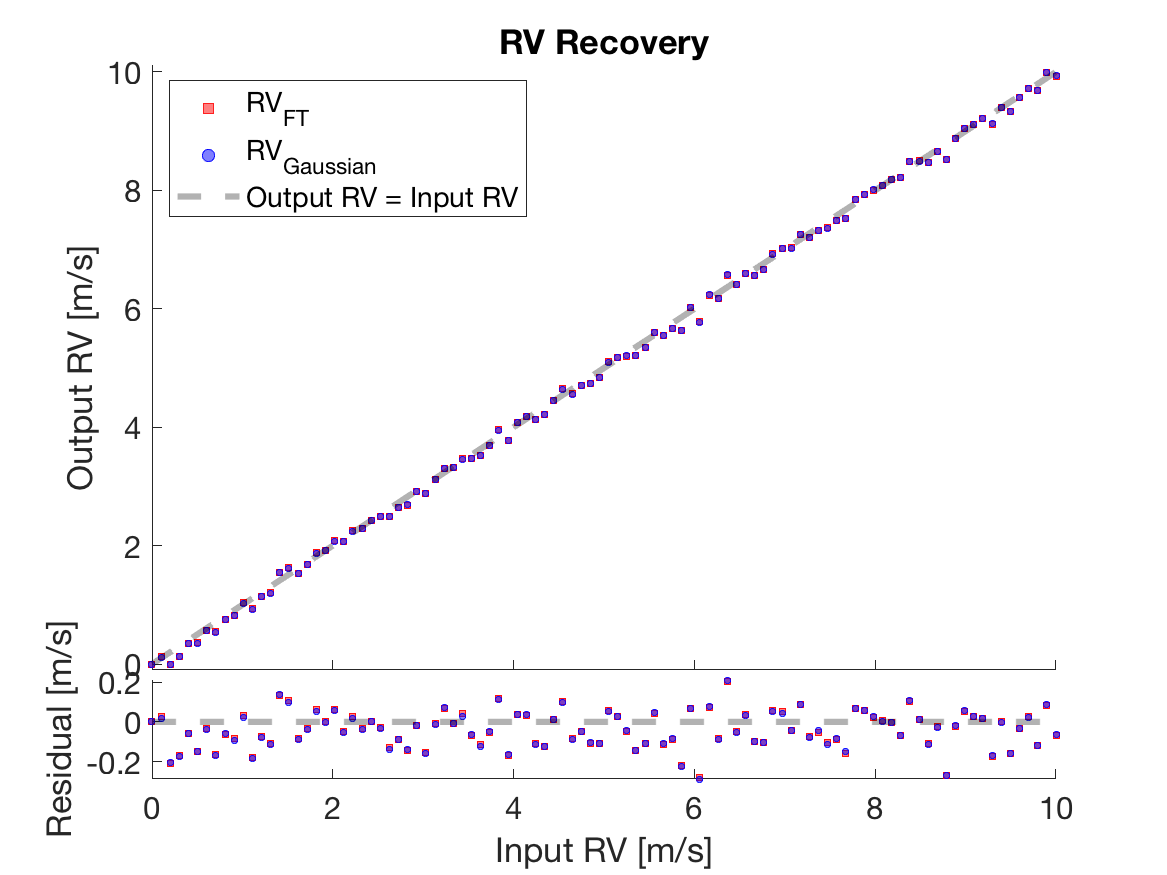
\includegraphics[width = 0.7 \linewidth]
{./Figures/Methods/5-LINE_SHIFT_ONLY.png}
\caption[Radial velocity recovery]
{Radial velocity recovery of line shifts with both methods: Fourier transform and Gaussian fit. Both results are highly consistent with each other. Errorbars are not plotted for clarity.}
\label{fig:rv_recovery}
\end{figure} 
%-------------
\FloatBarrier

%----------------------------------------------------------------------------------------	

\subsection{Further tests}
\label{sec:Further_tests}

Let's recall the justification of measuring a line shift in its Fourier space -- the shifting of a line (or a function), when viewed as shifting the sum of its Fourier basis functions (or any other basis functions), has equally the same amount of shift on every basis function, which can be measured as a phase shift in the Fourier phase spectrum. That is to say, utilising only part of the phase spectrum will also return the correct amount of shift of a line profile, although it is more likely to be affected by noise. The motivation of this practice will be discussed in \S\ref{sec:FT_ld} when it comes to line profile deformations, while we simply lay out the tests in this subsection. 

We choose to divide the whole frequency range into two parts (Fig.~\ref{fig:low-high-pass}) -- the lower frequency range (i.e. apply a low-pass filter) and the higher frequency range (i.e. apply a high-pass filter). The dividing frequency $\xi_{HL}$ is chosen such that both the lower and higher frequency ranges take up half of the power spectrum:\footnote{In practice, a cut-off frequency applies to the upper boundary of the high-pass filter. Frequencies higher than the cut-off frequency hardly contributes to the shape of the line profile as the power goes to 0, and they can be impacted by noise in a unpredictable way, although they are weighted by the nearly-zero power.}
\begin{equation}
	\int_{0}^{\xi_{HL}} P(\xi) d\xi = \int_{\xi_{HL}}^{+\infty} P(\xi) d\xi, 
\end{equation}
assuming the integration of power spectrum is a measurement of the amount of ``information", so that in a noise-free circumstance, we would put equal trust on the radial velocities obtained from the lower and higher frequencies. In the following, we use $RV_\text{FT,L}$ and $RV_\text{FT,H}$ to represent these two radial velocities.

%-------------
\begin{figure}[tbp]	
    \begin{subfigure}[b]{0.49\textwidth}
        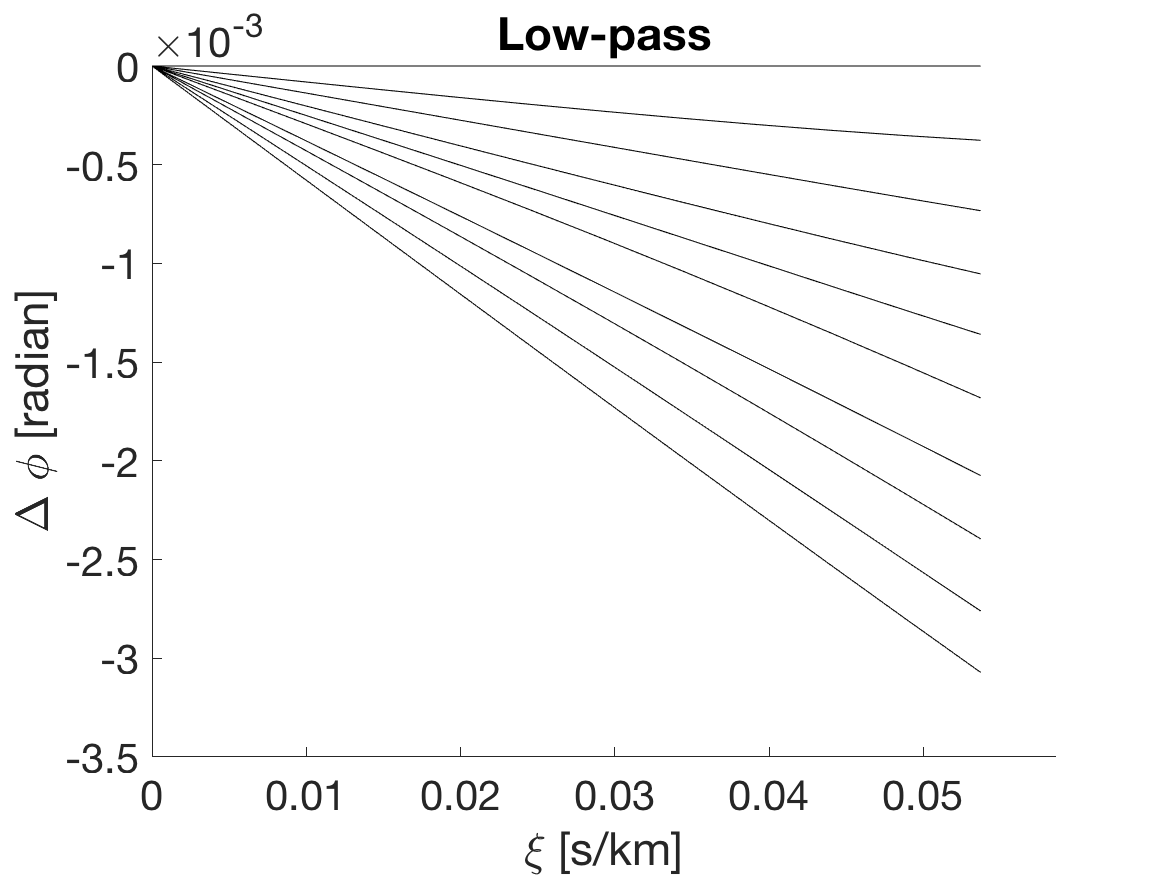
\includegraphics[width=\textwidth]{./Figures/Methods/4-Relative_phase_angle_L.png}
    \end{subfigure}
	~
    \begin{subfigure}[b]{0.49\textwidth}
        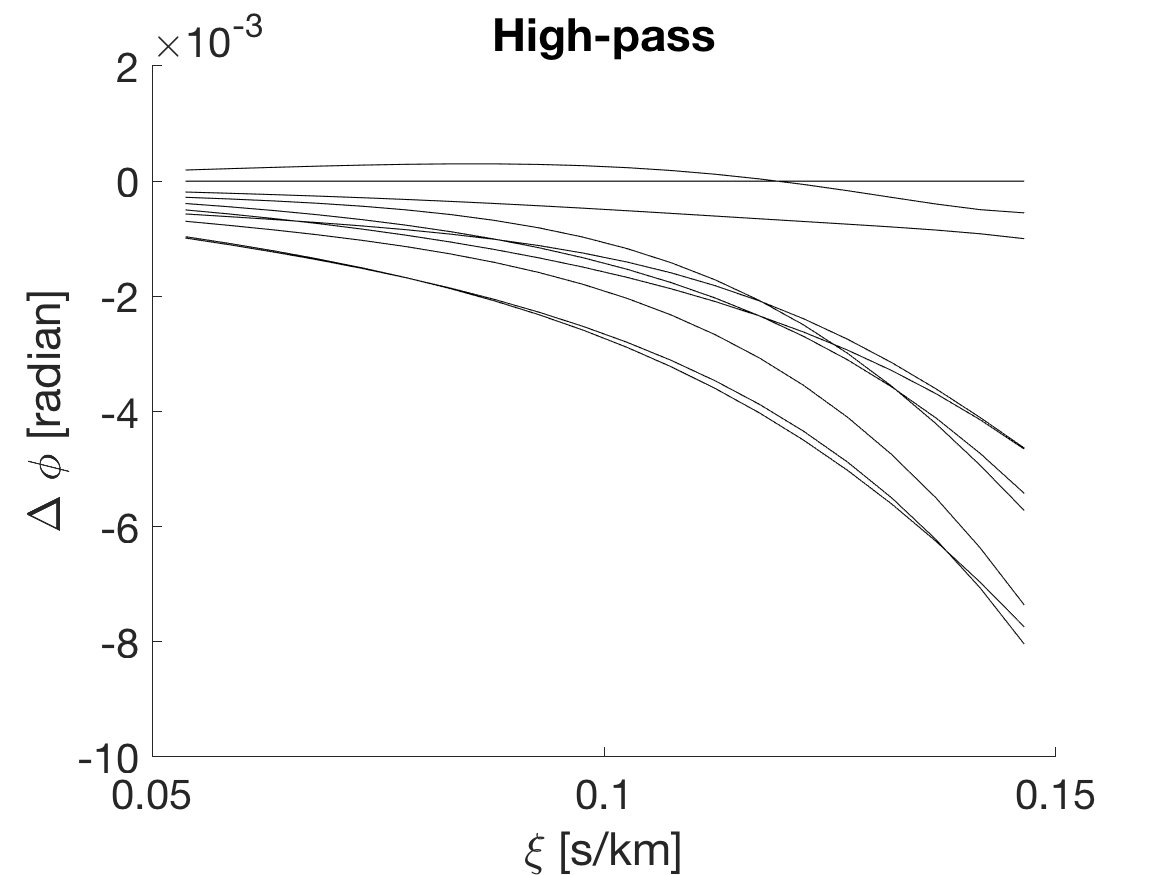
\includegraphics[width=\textwidth]{./Figures/Methods/4-Relative_phase_angle_H.png}
    \end{subfigure}	

    \caption[Low-pass and high-pass filters]
    {Differential phase spectrum as shown in Fig.~\ref{fig:dps} sub-divided into lower frequency range and higher frequency range. Only the non-negative ranges are plotted.}
\label{fig:low-high-pass}
\end{figure}    

Similar to Fig.~\ref{fig:rv_recovery} where we make use of the full range of frequencies, Fig.~\ref{fig:rv_recovery_LH} also presents a good 1:1 alignment between $RV_\text{FT,L}$, $RV_\text{FT,H}$ and the input radial velocity\footnote{The line of best fit presents a slope of $1.002\pm0.007$ for $RV_\text{FT,L}$ and $0.977\pm0.029$ respectively, with 95\% confidence bounds.}. The scatter of the residuals are $\sigma_\text{FT,L} = 0.11$ m/s and $\sigma_\text{FT,H} = 0.43$ m/s, seemingly contradicting with the expectation that equal amount of ``information" from which $RV_\text{FT,L}$ and $RV_\text{FT,H}$ are derived should deliver the same amount of scatter. The answer lies in the impact of noise (\S\ref{sec:noise}) -- higher frequency modes are more likely to be subjected to line deformations arising from stochastic behaviours, such as photon noise, stellar variability...

%-------------
\begin{figure}[tbp]
\centering
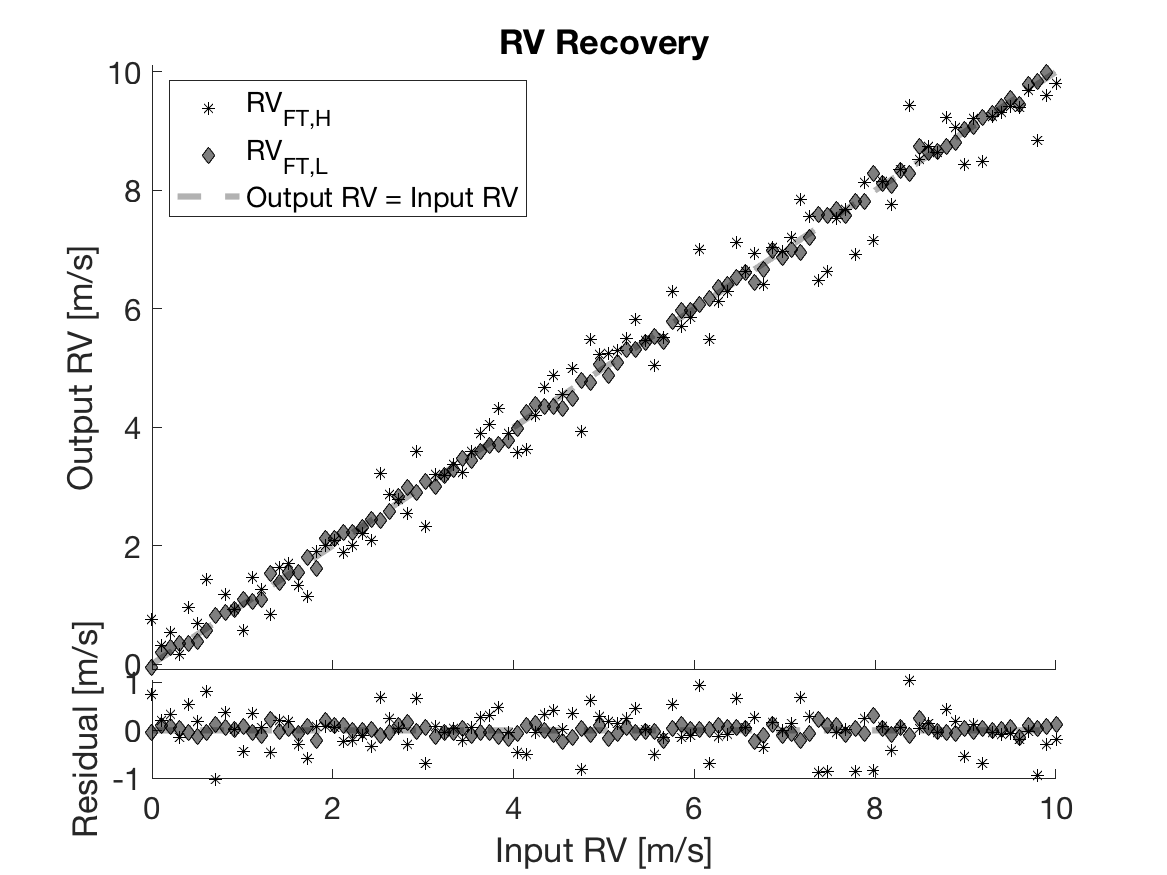
\includegraphics[width = 0.7 \linewidth]
{./Figures/Methods/5-LINE_SHIFT_ONLY-HL.png}
\caption[Low-pass and high-pass radial velocities]
{Radial velocity recovery of line shifts with low-pass and high-pass filters. Errorbars are not plotted for clarity.}
\label{fig:rv_recovery_LH}
\end{figure} 
%-------------
\FloatBarrier

%----------------------------------------------------------------------------------------
\subsection{Cut-off frequency}
\label{sec:noise}

We briefly mentioned in \S\ref{sec:Initial_tests} that the deviation from linearity in the differential phase spectrum arises from the photon noise injected in the simulated line profile, and in \S\ref{sec:Further_tests} that introducing a cut-off frequency in the upper boundary avoids dealing with excessive noise. This can be explained with the Fourier transformed line profile $\hat{h}(\xi)$ in a complex plane (also known as the Argand plane; Fig.~\ref{fig:FT_compelx_plane}). What we see is $\hat{h}(\xi)$ literally plotted on the complex plane -- of each complex number $\hat{h}(\xi)$, the argument returns the phase angle and the square of the absolute value returns the power, for that particular frequency $\xi$. For larger powers (i.e. $\hat{h}(\xi)$ far from the origin), the presence of noise hardly alters the phase angle; for lower powers (i.e. $\hat{h}(\xi)$ distributed in the vicinity of the origin), a slight displacement of $\hat{h}(\xi)$ in the complex plane means a considerable change in the phase angle. It justifies using the Fourier transform spectral power to be the weight of each frequency, and introducing a cut-off frequency when making a linear fit of the differential phase spectrum. 

Another possible reason for introducing the cut-off frequency is the periodicity of the basis functions in a Fourier transform. The basis function $e^{-2 \pi ix_0 \xi}$ repeats itself at the period of $1/\xi$, making measuring the shift longer than the order of $1/\xi$ degenerate because $x_0+k/\xi$ for $k\in\mathbb{Z}$ will give the same results. However, this is very unlikely the case that we may encounter. In the test examples above, the cut-off frequency is $\xi = 0.15$ s/km, corresponding to the period of $1/\xi\sim6.7$ km/s, way larger than the radial velocities induced by planets at m/s amplitudes. 

%-------------
\begin{figure}[tbp]	
    \begin{subfigure}[b]{0.49\textwidth}
        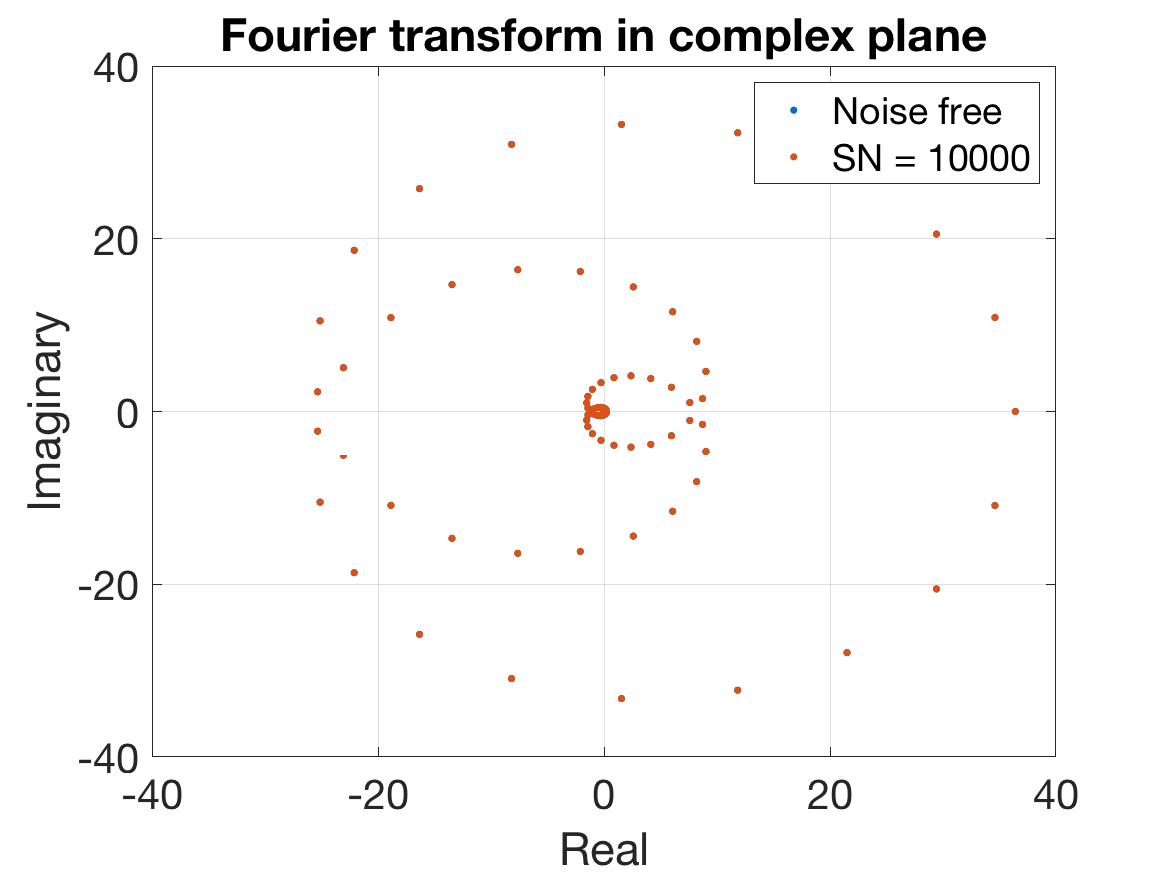
\includegraphics[width=\textwidth]{./Figures/Methods/7-Phase_angle_in_complex_plane_1.png}
%        \caption{Power spectrum (stacked)}
        \label{fig:FT_compelx_plane_1}
    \end{subfigure}
	~
    \begin{subfigure}[b]{0.49\textwidth}
        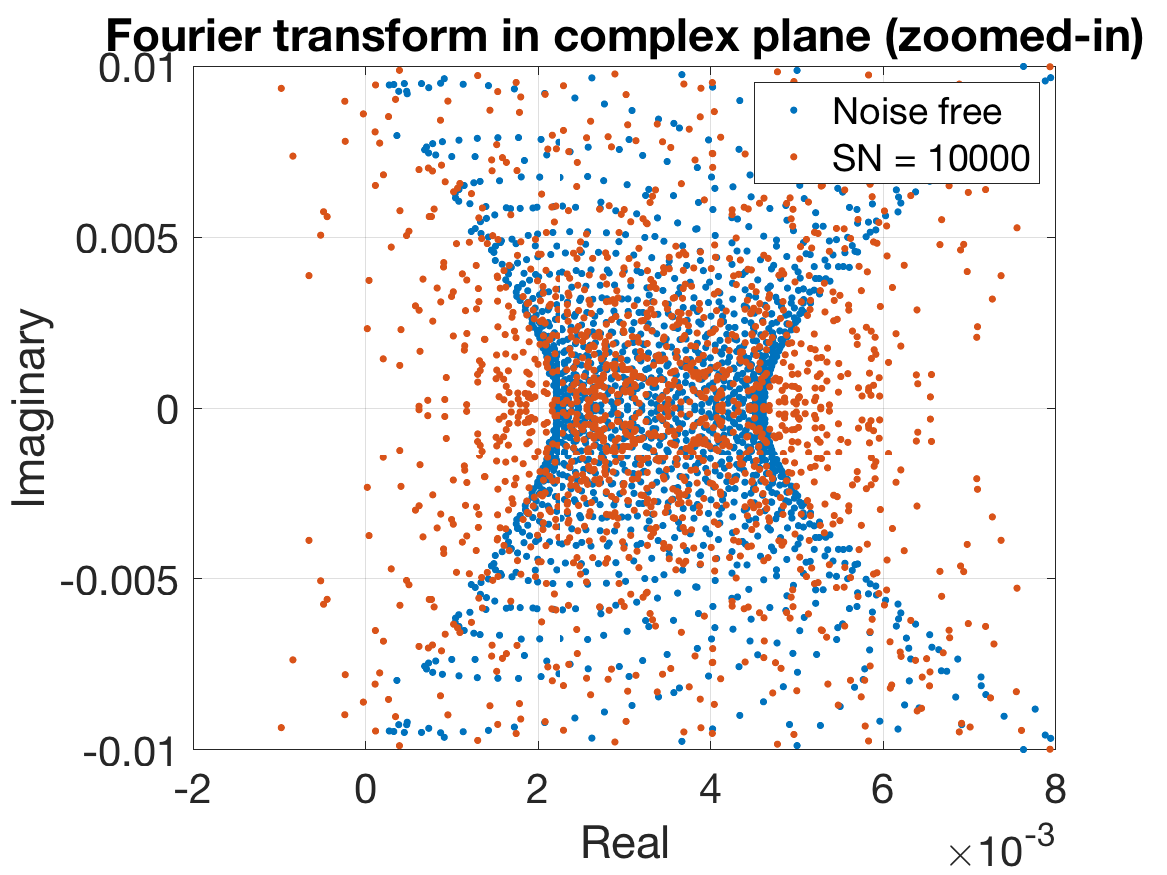
\includegraphics[width=\textwidth]{./Figures/Methods/7-Phase_angle_in_complex_plane_2.png}
%        \caption{Differential phase spectrum}
        \label{fig:FT_compelx_plane_2}
    \end{subfigure}	
    
    \caption[Fourier transform of a line profile in a complex plane]
    {The Fourier transform of a line profile in a complex plane. The right figure is a zoom-in of the left near the origin.}
\label{fig:FT_compelx_plane}
\end{figure}    
%-------------
\FloatBarrier

%This is because we only use part of the information from the original line profile -- both because we utilise a limited range of the differential phase spectra, and because we use only the phase spectra to measure this shift (ignoring the power spectra), while the total information in the original shifted line profile is contained in the combination of the power and phase spectra. 
%
%{\em CGT: This needs more work. You need to show the region you are not using to explain why you choose a more linited range, and
%then say why you chose that more limited range and justify it. Don't just say "higher frequency}.
%
%In fact, higher frequency range becomes useless 
%as the interpretation of Fourier transform in high frequencies is dominated by noise and does not represent the 
%intrinsic shift of the line profile any more. As a result, linearity of phase spectrum breaks down in higher frequencies. 
%The range of ``useful" frequencies will depend on the amount of noise (i.e. S/N). 

%----------------------------------------------------------------------------------------	

\subsection{Conclusion}
In this section, we have introduced a new method for measuring radial velocities -- Fourier phase spectrum analysis. The tests that we have made based on shifting a simulated line profile confirm our expectation that using the differential Fourier phase spectrum, it is possible to measure a radial velocity to similarly high precision. This provides an alternative to the traditional means of obtaining the radial velocities via centroiding the line profile in real space. 

In a broader context, this method will be applicable to measuring shifts of any pattern, and can be extended to higher dimensions. In this thesis, we primarily focus on its use to measure radial velocity shifts in spectral line profiles, and especially whether the Fourier transform phase velocity is more robust against the influence of changes in line deformation than traditional techniques.

\pagebreak
%----------------------------------------------------------------------------------------	
%----------------------------------------------------------------------------------------	

\section{Using the Fourier transform to probe line deformation}
\label{\thesection}
\label{sec:FT_ld}

In \S~\ref{ch:FT_line_shift}, we have tested that the Fourier phase spectrum analysis correctly measures the actual line profile shifts due to a bulk motion of the emitting star. In this section, we wish to test whether this method is more robust against spurious apparent radial velocity shifts produced by changes in the line profile shape in an emitting stars.

%----------------------------------------------------------------------------------------	

\subsection{Theory}
\label{sec:LD_Theory}

For a shift of a line profile by a small amount $x_0$, the same shift $x_0$ applies to \textit{all} of its basis functions. As for line deformation due to stellar variability, $x_0$ becomes frequency dependent \footnote{excluding the case where the result of a line deformation is exactly the same as a line shift, as this becomes indistinguishable by any means of studying the shape of the line profile alone}. That is to say, basis functions at different frequencies would be shifted by different amounts, resulting in shape changes (e.g. skewness) in the line profile. 
Therefore we modify the translation property of Fourier transform by rewriting $x_0$ as $x_0(\xi)$ in Eq.~\ref{eq:PhaseShift}:
\begin{equation}
	\Delta \phi(\xi) = -2 \pi x_0(\xi) \xi.
\label{eq:PhaseShift2_LPD}
\end{equation}
As a result, the local gradient of the differential phase spectrum becomes 
\begin{equation}
	\dv{(\Delta \phi)}{\xi} = -2 \pi (x_0 + \dv{x_0}{\xi}),
\label{eq:PhaseShift3_LPD}
\end{equation}
which reduces to Eq.~\ref{eq:gradient} when $x_0$ is a constant as in the case of a bulk line shift.
Note that the dependency of $\xi$ has been taken out of $\Delta \phi(\xi)$ and 
$x_0(\xi)$ in writing the differential equation above. 

In principle, we could numerically solve this differential equation based on the measured local gradient d$(\Delta \phi)$/d$\xi$ to obtain $x_0(\xi)$, but the local gradient measurement can be unreliable in the presence of noise. As a simplistic approach, we could use the \textit{averaged} shift $\overline{x_0(\xi)}$ of various frequency modes to describe different amounts of shift by rewriting Eq.~\ref{eq:PhaseShift2_LPD} as 
\begin{equation}
	\Delta \phi(\xi) = -2 \pi \overline{x_0(\xi)} \xi
\end{equation}
where $\overline{x_0(\xi)}$ is treated as a constant for the range of frequencies that we study. This concept will be helpful in describing the effective shifts applying the low-pass and high-pass filters when it comes to line deformation.
%if $x_0(\xi)$ changes with $\xi$ slowly within a certain frequency range,
%we can make the approximations that $x_0\sim$~const and d$x_0$/d$\xi\sim0$. With this, Eq.~\ref{eq:PhaseShift3_LPD} 
%converges back to Eq.~\ref{eq:gradient}.

%----------------------------------------------------------------------------------------	

\subsection{SOAP simulations}
\label{sec:Simulations}

In \S~\ref{ch:FT_line_shift}, we had used the SOAP simulator only to generate a line profile that resembles the HARPS observation. In this section, we would use the simulator SOAP~2.0 to study line deformations arising from starspots. 

Without loss of generality, we injected three spots with different longitudes, latitudes and sizes (parameters specified in Table~\ref{table:spot_configurations}) to model an emitting star, and generated 100 cross-correlation functions for the resulting  deformed line profiles evenly sampled throughout the rotation period of the star (Fig.~\ref{fig:line_profiles_deformation}). A very small amount of noise (equivalent to a S/N = 10,000) was also added into the line profiles for simulation demonstration purposes. 

%-------------
\begin{table}[htbp]
\centering
\begin{tabular}{|c|c|c|c|}
\hline 
 & Longitude & Latitude & Size in disk area percentage\\ 
\hline 
Spot 1 & $174^\circ$ & -$14^\circ$ & 0.18\% \\ 
\hline 
Spot 2 & $288^\circ$ & $74^\circ$  & 0.40\% \\ 
\hline 
Spot 3 & $51^\circ$  & $52^\circ$  & 0.50\% \\ 
\hline 
\end{tabular} 
\caption{Spot configurations}
\label{table:spot_configurations}
\end{table}
%-------------

%-------------
\begin{figure}[tbp]
    \begin{subfigure}[b]{0.49\textwidth}
        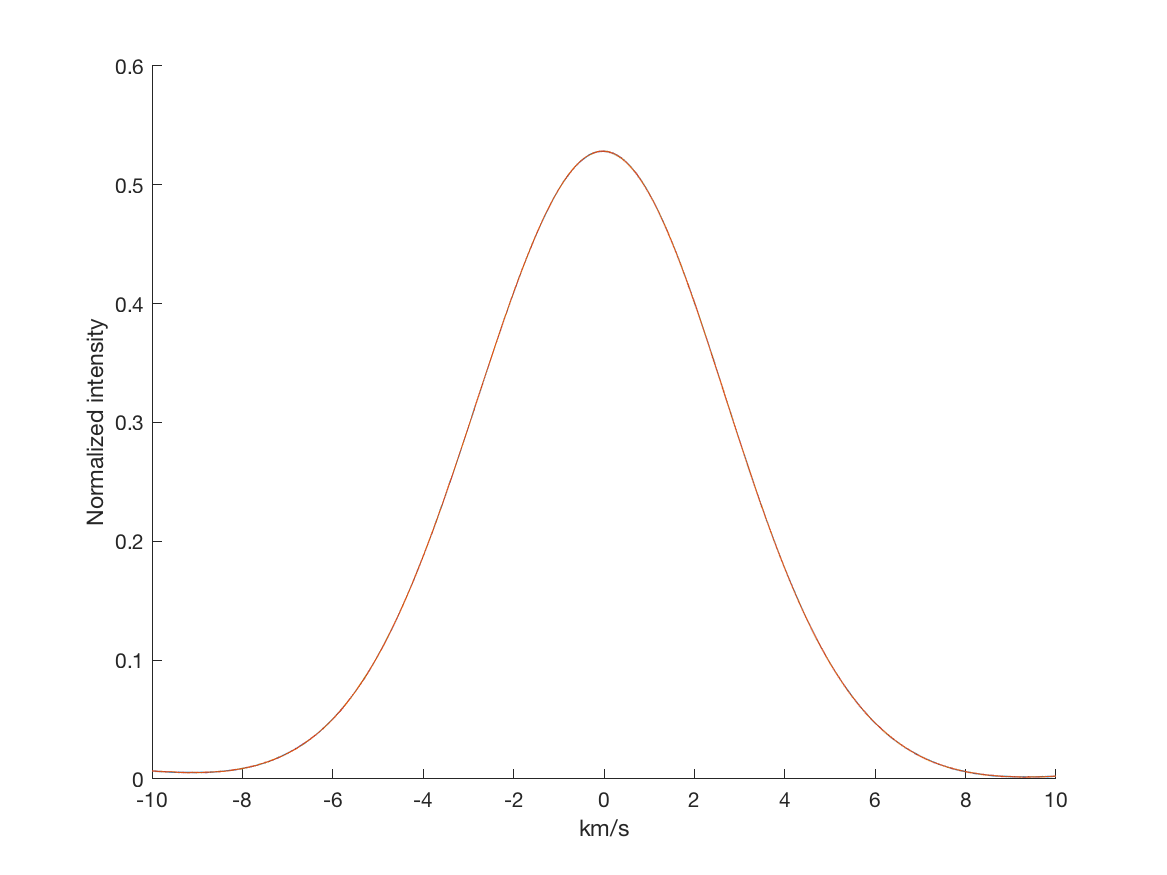
\includegraphics[width=\textwidth]{./Figures/Methods/LPD1-Line_Profile.png}
        \caption{Line profile (stacked)}
    \end{subfigure}
	~
    \begin{subfigure}[b]{0.49\textwidth}
        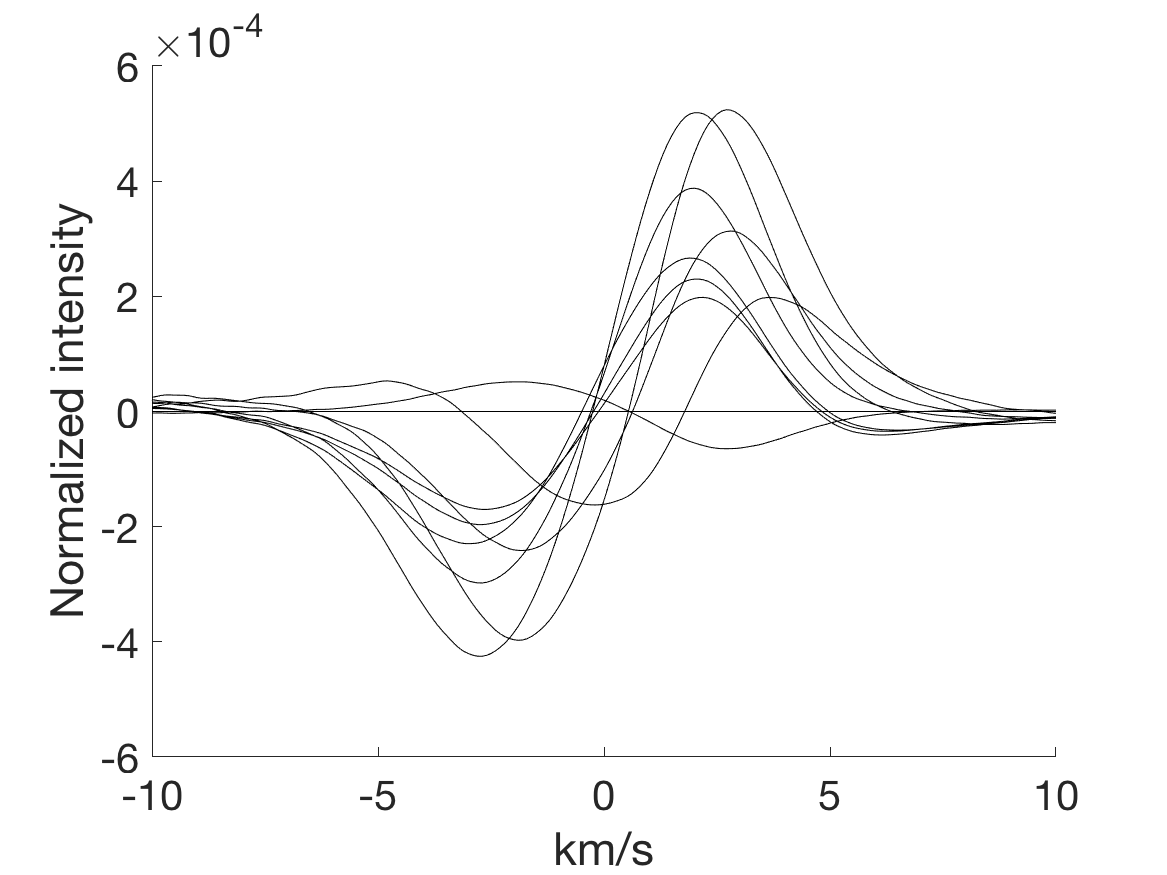
\includegraphics[width=\textwidth]{./Figures/Methods/LPD1-Differential_line_Profile.png}
        \caption{Differential line profile}
        \label{fig:ld_dlp}
    \end{subfigure}	
    
    \caption[Deformed line profile]{Deformed line profile. For the sake of clarity, the differential line profiles are plotted noise-free and only 10 out of 100 profiles are presented.}
\label{fig:line_profiles_deformation}
\end{figure}	
%-------------
\FloatBarrier

%----------------------------------------------------------------------------------------	
\subsection{Fourier phase spectrum analysis}

\subsubsection{$RV_\text{FT}$}
We then take the same approach as in  \S~\ref{ch:FT_line_shift} to obtain the power spectrum and the differential phase spectrum (Fig.~\ref{fig:FT_process_LPD}) to recover the radial velocities $RV_\text{FT}$. It notes, line deformation contributes to a skewed differential phase spectrum, as predicted in \S\ref{sec:LD_Theory}. 

%-------------
\begin{figure}[tbp]	
    \begin{subfigure}[b]{0.49\textwidth}
        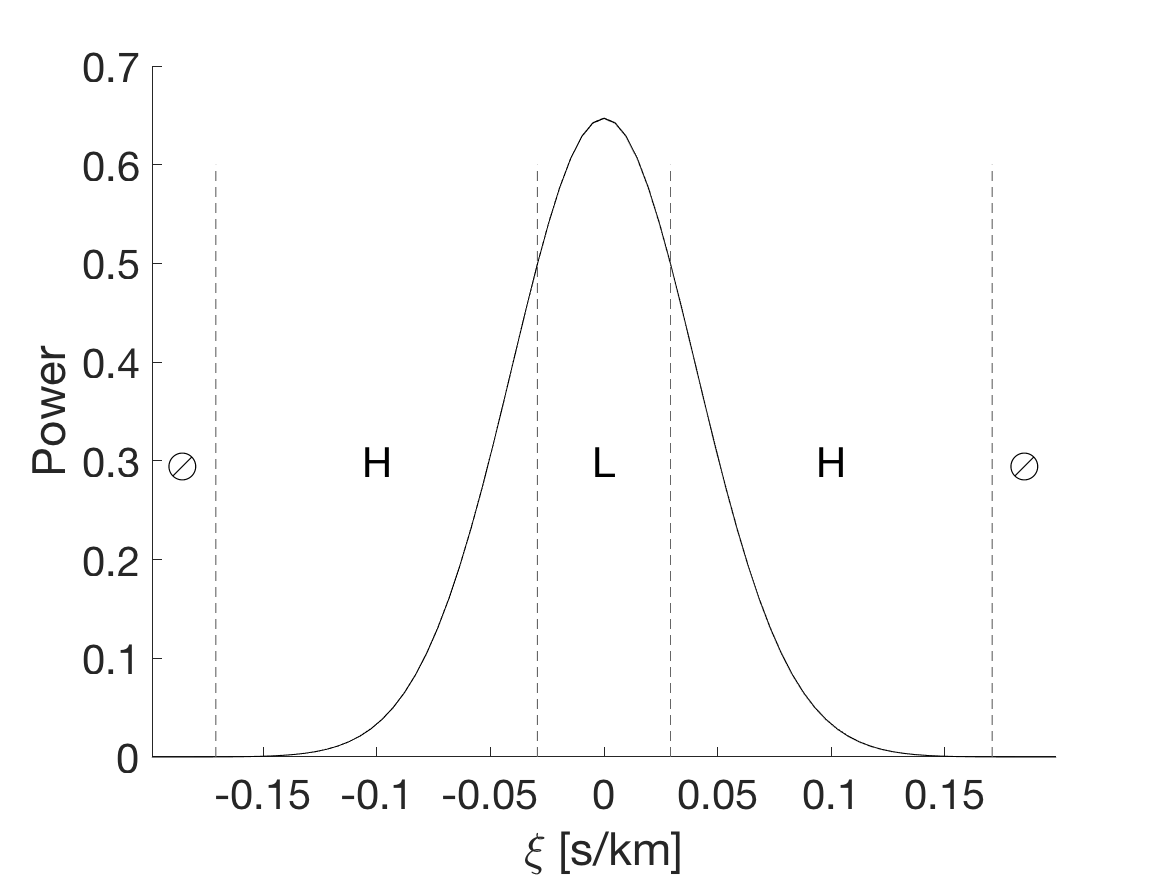
\includegraphics[width=\textwidth]{./Figures/Methods/LPD2-FT_power.png}
        \caption{Power spectrum (stacked)}
    \end{subfigure}
	~
    \begin{subfigure}[b]{0.49\textwidth}
        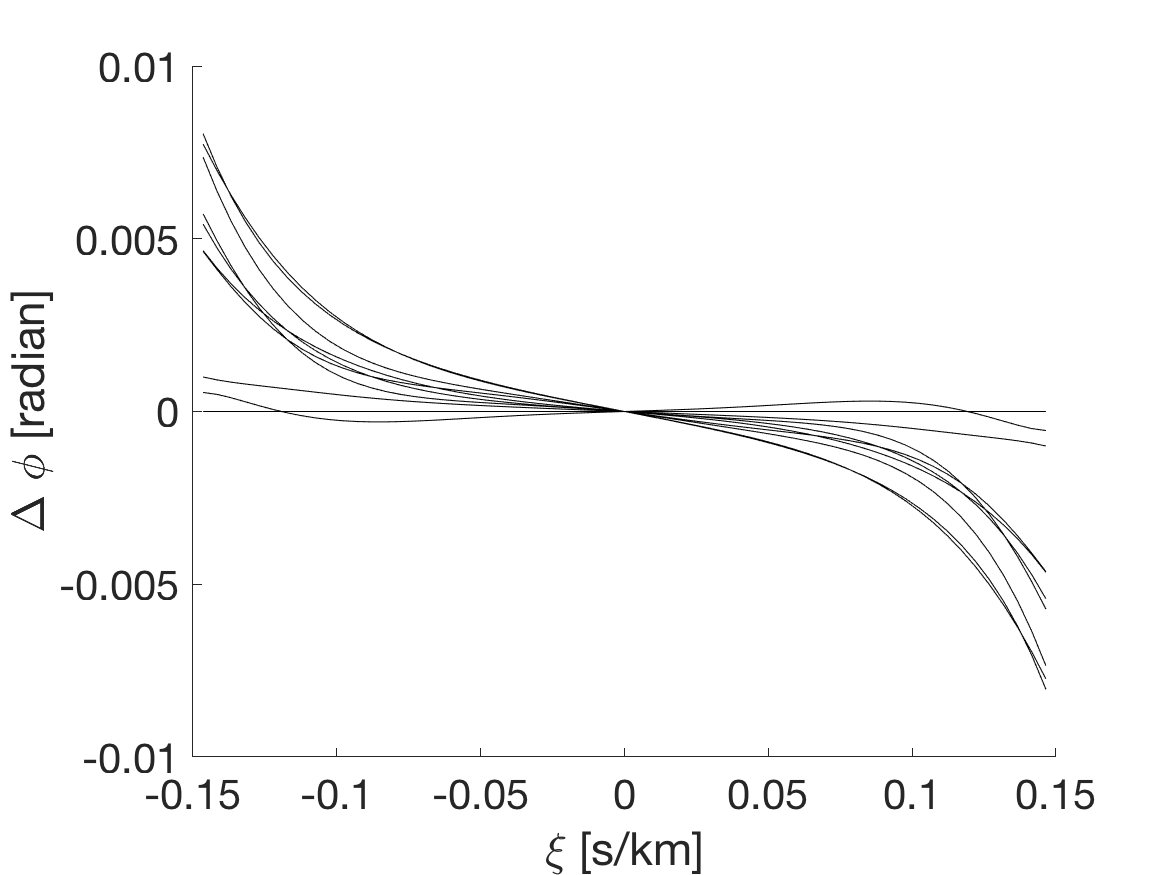
\includegraphics[width=\textwidth]{./Figures/Methods/LPD4-Relative_phase_angle.png}
        \caption{Differential phase spectrum}
        \label{fig:dps_LPD}
    \end{subfigure}	
    
    \caption[Fourier transform of deformed line profile]
    {Fourier transform of deformed line profile. Only 10 out of 100 differential phase spectra are presented.}
\label{fig:FT_process_LPD}
\end{figure}    
%-------------

In this case, the input radial velocities would be the apparent radial velocities of deformed line profiles (also known as jitter). Both velocities $RV_\text{FT}$ and $RV_\text{Gaussian}$ are plotted against rotation phase (Fig.~\ref{fig:rv_recovery_deformed}). If we take the root-mean-squares of both $RV_\text{FT}$ and $RV_\text{Gaussian}$ to be the intrinsic noise level ($\sigma_\text{FT} = \sigma_\text{Gaussian} = 0.08$ m/s) corresponding S/N = 10,000, the uncertainty of $RV_\text{FT} - RV_\text{Gaussian}$ as residual would have an uncertainty of 
$\sqrt{\sigma_\text{FT}^2+\sigma_\text{Gaussian}^2}\approx0.11$ m/s. As $\mid RV_\text{difference}\mid = \mid RV_\text{FT} - RV_\text{Gaussian}\mid < 0.03$ m/s, we can agree that $RV_\text{FT}$ and $RV_\text{Gaussian}$ are indistinguishably consistent. 

%-------------
\begin{figure}[tbp]
\centering
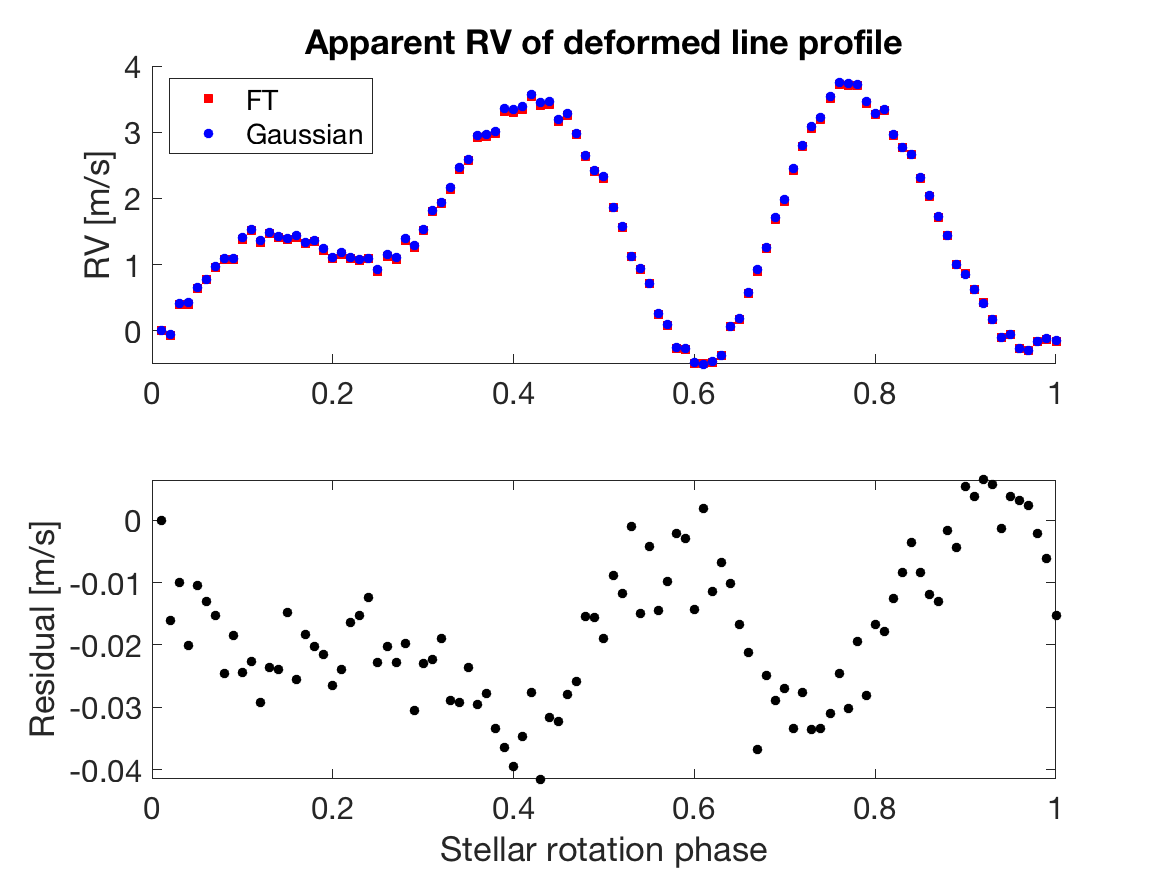
\includegraphics[width = 0.7 \linewidth]
{./Figures/Methods/5-JITTER_ONLY_3.png}
\caption[Apparent RV of deformed line profile]
{Apparent RV of deformed line profile calculated with Fourier transform and Gaussian fit. Both results are also highly consistent with each other. $RV_\text{difference} = RV_\text{FT} - RV_\text{Gaussian}$.}
\label{fig:rv_recovery_deformed}
\end{figure} 
%-------------
\FloatBarrier

To conclude, the Fourier phase spectrum analysis, using (almost) all the information in the power spectrum and the phase spectrum, returns highly consistent radial velocities as the line centroid acquiring by fitted a Gaussian profile. This consistency applies both for measuring a direct line shift and an apparent shift of a deformed line profile. 

%----------------------------------------------------------------------------------------	
\subsubsection{$RV_\text{FT,H}$ and $RV_\text{FT,L}$}
\label{subsec:FT,HL}

Although the intrinsic line deformation (in the absence of any velocity shift in the host star) does mimic the radial velocity shift, we note the shape differences in the differential phase spectrum between an actual line shift (Fig.~\ref{fig:dps}) and a line deformation (Fig.~\ref{fig:dps_LPD}) -- the latte presents relatively flat features in lower frequencies and becomes more skewed towards higher frequencies. Such differences provide key messages to differentiate the two circumstances.

According to \S\ref{sec:LD_Theory} where we introduced $\overline{x_0(\xi)}$ -- an averaged shift of a particular frequency range -- we can therefore compute the equivalent radial velocity shift for each of the lower and higher frequency ranges (Fig.~\ref{fig:low-high-pass_lpd}), denoted as $RV_\text{FT,L}$ and $RV_\text{FT,L}$ respectively. 

%-------------
\begin{figure}[tbp]	
    \begin{subfigure}[b]{0.49\textwidth}
        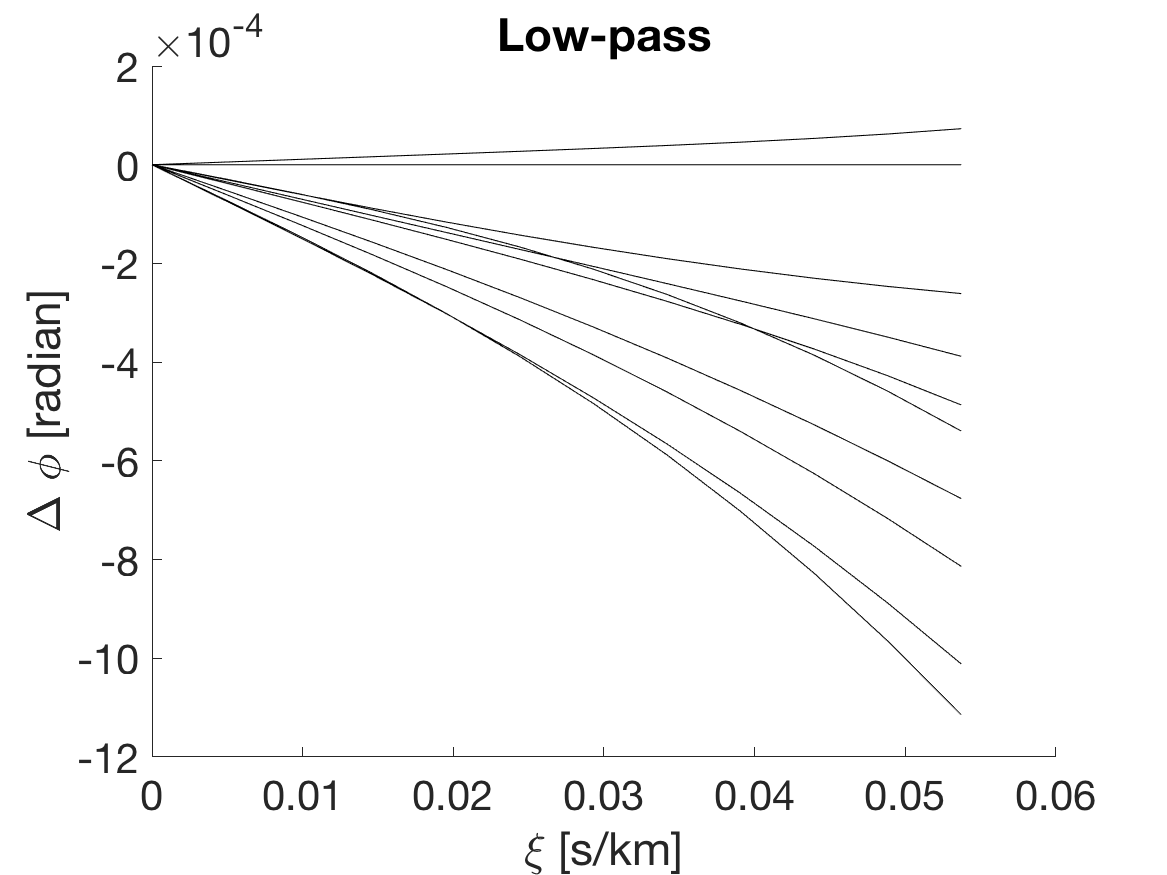
\includegraphics[width=\textwidth]{./Figures/Methods/LPD4-Relative_phase_angle_L.png}
%        \caption{Power spectrum (stacked)}
    \end{subfigure}
	~
    \begin{subfigure}[b]{0.49\textwidth}
        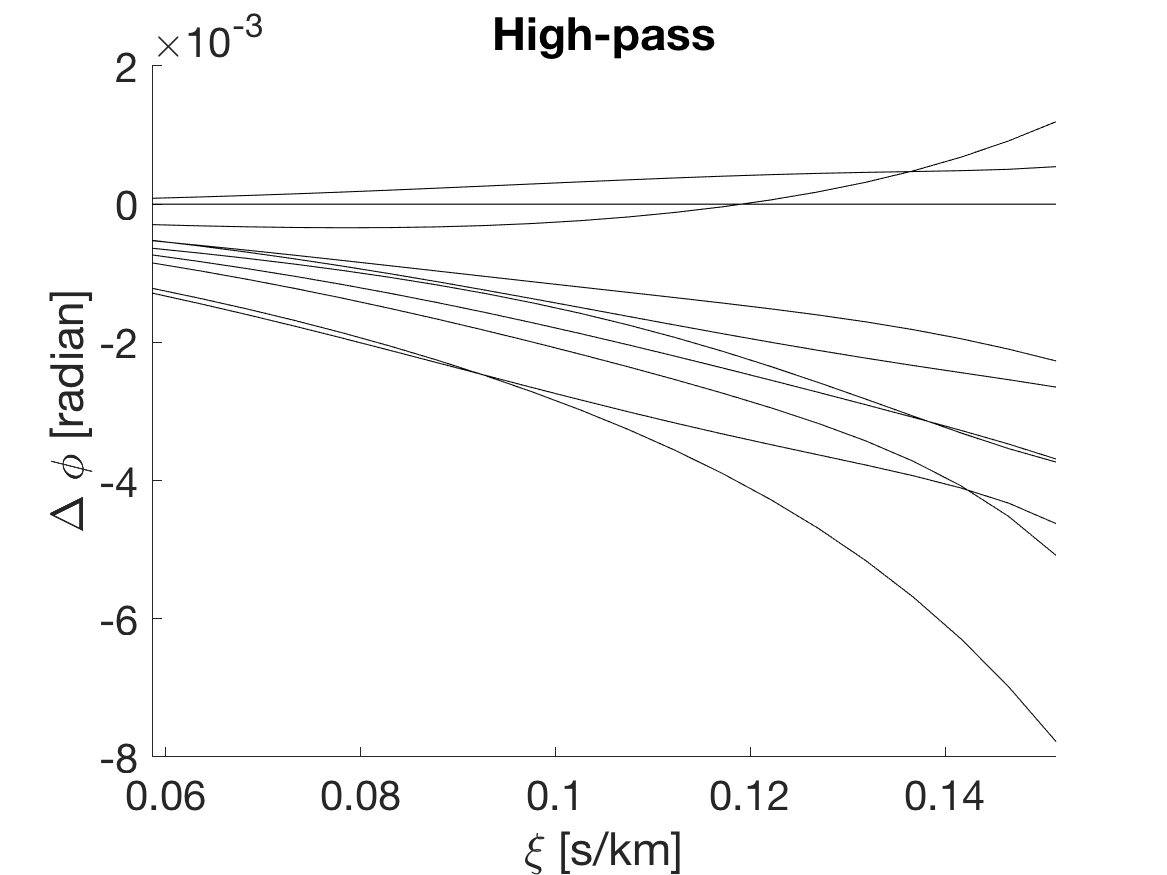
\includegraphics[width=\textwidth]{./Figures/Methods/LPD4-Relative_phase_angle_H.png}
%        \caption{Differential phase spectrum}
    \end{subfigure}	
    
    \caption[Low-pass and high-pass filters]
    {Differential phase spectrum as shown in Fig.~\ref{fig:dps_LPD} sub-divided into lower frequency range and higher frequency range. Only the non-negative ranges are plotted.}
\label{fig:low-high-pass_lpd}
\end{figure}    
%-------------

To present our results, we plot the obtained $RV_\text{FT,L}$ and $RV_\text{FT,L}$ against the jitter (line centroid fitted by a Gaussian profile) in Fig.~\ref{fig:FT_vs_Gaussian}. The $RV_\text{FT,L}$ and $RV_\text{FT,L}$ can be clearly clustered into two groups, both linearly correlated with the jitter, and yet neither has a 1:1 correlation. $RV_\text{FT,H}$ demonstrates a higher response to jitter. Fitting with a linear regression model, it comes with a slope $k_\text{H} = 1.978\pm0.100$, meaning an apparent radial velocity shift of 1 m/s due to line deformation is detected as $1.978\pm0.100$ m/s shift on average using \textit{this} high-pass filter; whereas the slope for applying a low pass filter is $k_\text{L} = 0.847\pm0.015$, meaning $RV_\text{FT,L}$ is less sensitive to the line profile deformation. When combining both filters, we would have obtained $RV_\text{FT}$, the same response to jitter, as shown in Fig.~\ref{fig:rv_recovery_deformed}.

%-------------
\begin{figure}[tbp]
\centering
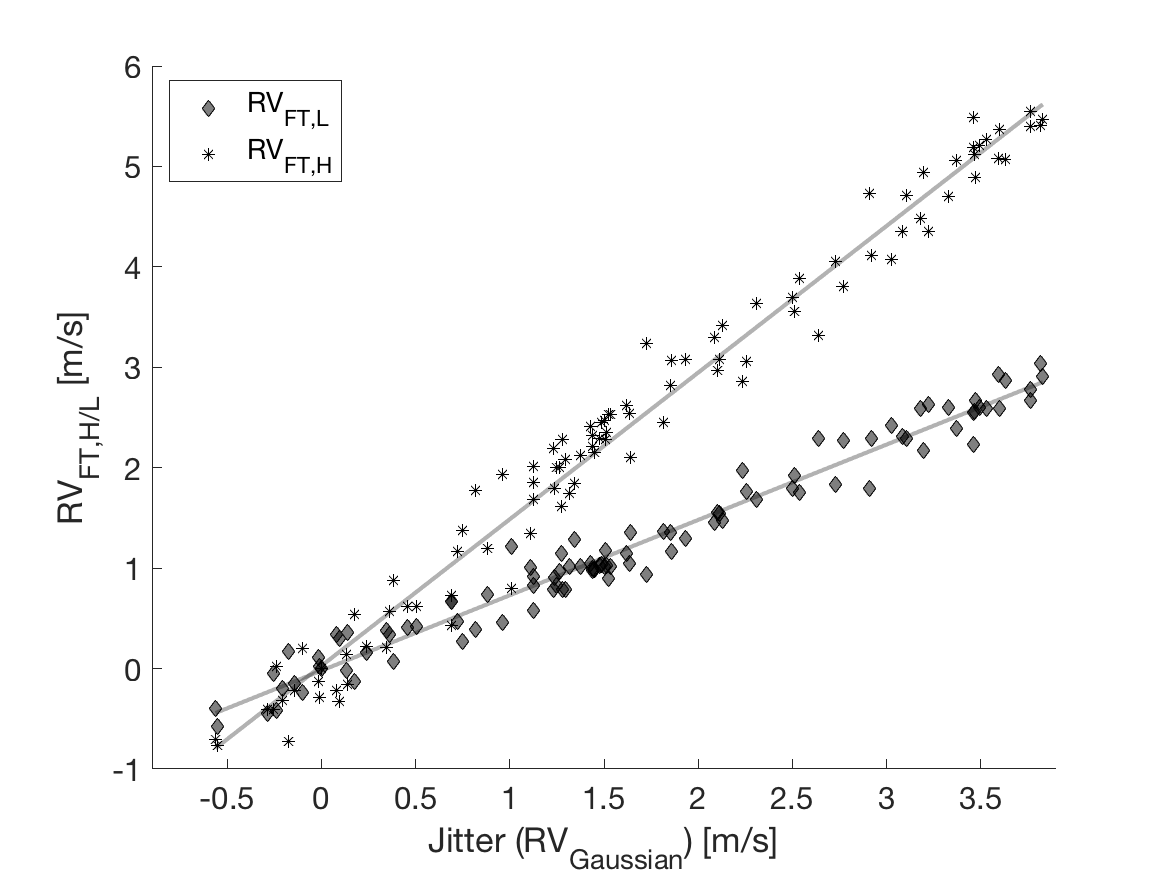
\includegraphics[width = 0.7 \linewidth]
{./Figures/Methods/5-JITTER_ONLY_1.png}
\caption[Fourier transform in response to line deformation]
{Applying the low-pass and high-pass filters, the Fourier transform $RV_\text{FT,L}$ and $RV_\text{FT,H}$ are linearly correlated with the jitter ($RV_\text{Gaussian}$).}
\label{fig:FT_vs_Gaussian}
\end{figure} 
%-------------

We could further investigate how well this linearity behaves for each filter by scaling the measured $RV_\text{FT,L}$ and $RV_\text{FT,H}$ by their corresponding factors $1/k_\text{L}$ and $1/k_\text{H}$ respectively, and compare them with the jitter ($RV_\text{Gaussian}$), as presented in Fig.~\ref{fig:scaling_RV_FT}. The root-mean-squares of the residuals ($RV_\text{FT,L/H}/k_{L/H} - RV_\text{Gaussian}$) are $\sigma_\text{FT,L} \approx 0.11$ m/s and $\sigma_\text{FT,H} \approx 0.31$ m/s respectively. The reason for $\sigma_\text{FT,H}>\sigma_\text{FT,L}$ is the same as mentioned in \S\ref{sec:Further_tests}, being higher frequency modes are more affected by noise. 

%-------------
\begin{figure}[tbp]
\centering
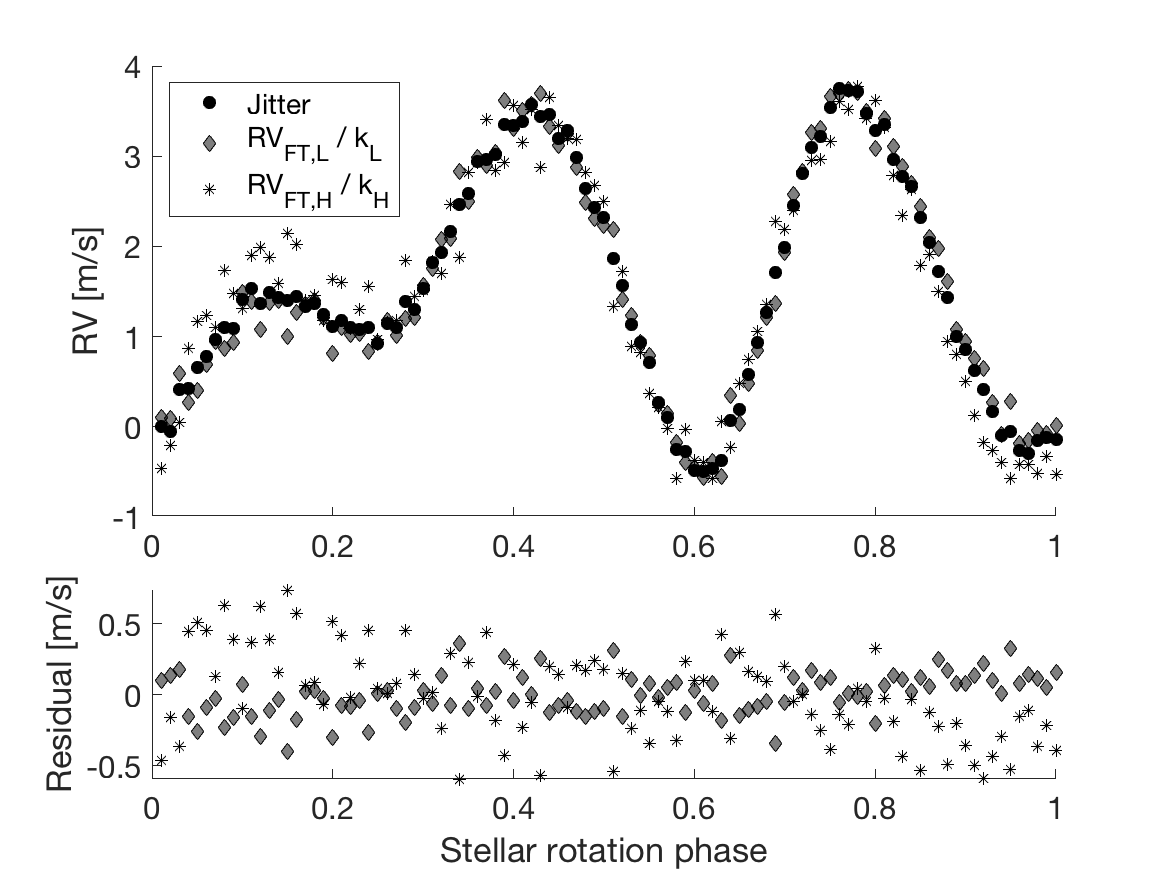
\includegraphics[width = 0.7 \linewidth]
{./Figures/Methods/5-JITTER_ONLY_4.png}
\caption[Scaling the low-pass and high-pass Fourier transformed radial velocities]
{Scaling the low-pass and high-pass Fourier transformed radial velocities to match the input jitter.}
\label{fig:scaling_RV_FT}
\end{figure} 
%-------------

To conclude this subsection, the apparent radial velocity shift due to spectral line deformation (i.e. jitter) can be seen as a mingle of two radial velocities -- $RV_\text{FT,H}$ and $RV_\text{FT,L}$ -- one in higher frequency modes the other in lower frequency modes. They are both, as obtained from the simulated spectral line profiles, scaled linearly with jitter.

%An intuitive way to understand why 
%
%If we compare the differential phase spectra in Fig.~\ref{fig:FT_process} and Fig.~\ref{fig:FT_process_LPD},
%it is quite obvious that the differential phase spectrum of a deformed line profile is no longer linear 
%due to the $x_0$ dependency on $\xi$, as we discussed in \S~\ref{sec:LD_Theory}. Nevertheless, applying the 
%local linear approximation can provide a radial velocity shift for that frequency range. We will primarily 
%use the lower frequency range (from -0.06 to 0.06~(km/s)$^{-1}$ in this case) for the reasons that 
%it is where information is mostly concentrated and that it is less noise-sensitive. {\em CGT: Sorry, 
%but you still haven't demonstrated this sufficiently}
%
%However, the differential phase shift at lower frequency is {\em less} sensitive to the
%influence of line profile deformation. 
%If we concentrate on frequencies in the range $\mid\xi\mid < 0.06$ (km/s)$^{-1}$ (sensitive to line profile
%structure at  velocities $> 1/\mid\xi\mid = 16$ km/s) we find that these lower frequency modes are
%less effectively modulated by the higher frequency line deformations, as shown in the 
%differential line profile in Fig.~\ref{fig:ld_dlp}. 
%
%In addition, the slope $k$ will change depending on the 
%frequency range in which the linear regression model is applied. 
%For example, if we select the higher frequency range in the differential phase spectrum, we will 
%expect larger $RV_\text{FT}$ and hence a larger $k$ in general. 
%
%{\em CGT: I tried to rewrite the above, but I'm not convinced either the text or the figures are
%very clear! In partiuclar you need a clear and compelling demosntration why you've chosen the lower
%frequency range you have}

%----------------------------------------------------------------------------------------	
\subsection{Jitter model}
\label{subsec:Jitter_model}

We have found in \S~\ref{ch:FT_line_shift} that the following measurable quantities demonstrate basically the same response to pure line shifts: $RV_\text{FT}$ derived from the whole frequency range, $RV_\text{FT,H}$ from the higher frequency range, $RV_\text{FT,L}$ from the lower frequency range and $RV_\text{Gaussian}$ being the line centroid fitted by a Gaussian profile  We have also found in this section (\S~\ref{sec:FT_ld}) so far, that both $RV_\text{FT,H}$ and $RV_\text{FT,L}$ are linearly correlated with the jitter, to which $RV_\text{FT,H}$ is more sensitive ($k_\text{H}>1$) and $RV_\text{FT,L}$ is less sensitive ($k_\text{L}<1$). 

We can therefore write the following measurable quantities -- $RV_\text{Gaussian}$ (or $RV_\text{FT}$), $RV_\text{FT,L}$ and $RV_\text{FT,H}$ -- as the sum of corresponding contributions from a bulk shift in the star (which we hereafter assume to be due to a planet or planets), and variability in the stellar line profile (hereafter lumped under the general name ``jitter'')\footnote{For writing in elegance, a constant offset term for each of the equations is taken out in all of the following equations in this subsection.}:
\begin{align}
	RV_\text{Gaussian} 	&= RV_\text{planet} + RV_\text{jitter}				 \label{eq:RV_Gau} \\
	RV_\text{FT,L} 		&= RV_\text{planet} + k_L \cdot RV_\text{jitter} 		 \label{eq:RV_FTL} \\
	RV_\text{FT,H} 		&= RV_\text{planet} + k_H \cdot RV_\text{jitter}.		 \label{eq:RV_FTH}
\end{align}
Subtracting one from the other to remove $RV_\text{planet}$ and reduce to two independent equations
\begin{align}
	RV_\text{Gaussian} - RV_\text{FT,L} 	&= (1-k_L) \cdot RV_\text{jitter}\\
	RV_\text{FT,H} - RV_\text{Gaussian}	&= (k_H-1) \cdot RV_\text{jitter}
\end{align}
Rearranging yields two expressions of the jitter model
\begin{align}
	RV_\text{jitter} &= \frac{RV_\text{Gaussian} - RV_\text{FT,L}}{1-k_L} 	\label{eq:jitter_model1} \\
	RV_\text{jitter} &= \frac{RV_\text{FT,H} - RV_\text{Gaussian}}{k_H-1}		\label{eq:jitter_model2} 
\end{align}
where $RV_\text{Gaussian}, RV_\text{FT,L}$ and $RV_\text{FT,H}$ are direct measurements, whereas $k_L$ and $k_H$ are unknowns\footnote{We could determine $k_L$ and $k_H$ in the demonstrated simulations only because we knew the jitter.}. Dividing the two equations above further cancels $RV_\text{jitter}$, leaving 
\begin{equation}
	\frac{RV_\text{Gaussian}-RV_\text{FT,L}}{RV_\text{FT,H} - RV_\text{Gaussian}} = \frac{1-k_L}{k_H-1},
\end{equation}
which means $(1-k_L)/(1-k_H)$ can now be robustly obtained by fitting a linear regression model on $(RV_\text{Gaussian}-RV_\text{FT,L})$ against $(RV_\text{Gaussian} - RV_\text{FT,H})$. With this, we rewrite the jitter model in a unified form -- the weighted sum of the two jitter expressions from Eq.~\ref{eq:jitter_model1} and Eq.~\ref{eq:jitter_model2}: 
\begin{align*}
	RV_\text{jitter} &= w_1 \frac{RV_\text{Gaussian} - RV_\text{FT,L}}{1-k_L} + w_2 \frac{RV_\text{FT,H}-RV_\text{Gaussian}}{k_H-1} \\
	&= \frac{1}{{k_H-1}} \bigg[w_1 \frac{RV_\text{Gaussian} - RV_\text{FT,L}}{\frac{1-k_L}{k_H-1}} + w_2 (RV_\text{FT,H}-RV_\text{Gaussian})\bigg] \\
	&= \alpha \bigg[w_1 \frac{RV_\text{Gaussian} - RV_\text{FT,L}}{\frac{1-k_L}{k_H-1}} + w_2 (RV_\text{FT,H}-RV_\text{Gaussian})\bigg] \numberthis \label{eq:jitter_model_final}
\end{align*}
in which the weights satisfy $w_1+w_2=1$ and $1/(k_H-1)$ is replaced by the scaling factor $\alpha$ in the last step. 

Additionally, we can roughly estimate the uncertainty of $RV_\text{jitter}$ in Eq.~\ref{eq:jitter_model1} and Eq.~\ref{eq:jitter_model2} by treating $RV_\text{Gaussian}$, $RV_\text{FT,L}$ and $RV_\text{FT,H}$ are independent variables, and $k_{L/H}$ is a constant: 
\begin{align}
	\Delta RV_\text{jitter,L} &\approx \frac{\sqrt{\sigma_\text{Gaussian}^2 + \sigma_\text{FT,L}^2}}{1-k_L} \\
	\Delta RV_\text{jitter,H} &\approx \frac{\sqrt{\sigma_\text{Gaussian}^2 + \sigma_\text{FT,H}^2}}{k_H-1}.
\end{align}
Substituting the following values: $\sigma_\text{Gaussian} = 0.08$ m/s (\S\ref{sec:Initial_tests}), $\sigma_\text{FT,L} = 0.11$ m/s and $\sigma_\text{FT,H} = 0.43$ m/s (\S\ref{sec:Further_tests}), $k_L = 0.847$ and $k_H = 1.978$ (\S\ref{subsec:FT,HL}), we obtain $\Delta RV_\text{jitter,L} = 0.89$ m/s and $\Delta RV_\text{jitter,H} = 0.45$ m/s.


% but can be incorporated into the radial velocity models (i.e. substitute $RV_\text{jitter}$ in Eq.~\ref{eq:RV_Gau} by either Eq.~\ref{eq:jitter_model1} or Eq.~\ref{eq:jitter_model2}) in the process of recovering planets.


When there's no planet or the planetary radial velocity signal is negligible compared with the size of jitter, $RV_\text{FT,L}$ and $RV_\text{FT,H}$ will be proportional to $RV_\text{jitter}$ (Example: \S\ref{sec:HD189733}).

%----------------------------------------------------------------------------------------	
\subsection{Testing the recovery of jitter}
\label{sec:check}

We again performed tests to see if we can correctly recover artificially generated jitter using our new technique (Eq.~\ref{eq:jitter_model_final}).

We generated 200 deformed line profiles (in the form of cross-correlation functions) using SOAP~2.0. All the configurations are the same as used in \S\ref{sec:Simulations}, except that the data are produced from two rotation periods instead of one. The jitter amplitude is roughly 2 m/s. In addition, each line profile is further shifted by an amount $RV_\text{planet}$ appropriate for a planet generating a Keplerian orbit in the star of the amplitude\footnote{In principle, the $RV_\text{planet}$ configuration shouldn't matter in producing the jitter model because it is cancelled out in the jitter model as derived in \S\ref{subsec:Jitter_model}.}: $A_\text{planet} = 2~\text{m/s}$. The planetary orbital period to stellar rotation period ratio is set to be 0.7 (i.e. $P_\text{rot}/P_\text{orb} =\nu_\text{orb}/\nu_\text{rot}= 0.7$). 

We then obtain three sets of radial velocities for each simulated profile: $RV_\text{Gaussian}$, $RV_\text{FT,H}$ and $RV_\text{FT,L}$ (Fig.~\ref{fig:PLANET_AND_JITTER} upper panel). We test three different combinations of $w_1$ and $w_2$ and apply a scaling factor $\alpha$ (fitted by linear regression to the known input jitter) to see how well it matches the input jitter: (1) $w_1=1, w_2=0$; (2) $w_1=0.5, w_2=0.5$; (3) $w_1=0, w_2=1$. To visually show the trends of these three test jitter models, a moving average modulated by a Gaussian kernel is implemented to smooth out the data (Fig.~\ref{fig:PLANET_AND_JITTER} middle panel). All these three sets of jitter model successfully recover adequate information of the input jitter, while presenting minor difference among each other. 

To quantitatively examine their performance, we compare the scatter of the input jitter $\sigma_\text{jitter}$ and that of the difference between the input jitter and the jitter models $\sigma_\text{residual}$. The former can be treated as the scatter after fitting the correct planet(s) without jitter correction, while the latter can be treated as the scatter after the additional jitter is removed. Table~\ref{table:jitter_model_scatter} lays out the scatter $\sigma_\text{residual}$ for the raw jitter models and the smoothed jitter models. The smoothed jitter can be useful in reducing the larger scatter of radial velocities obtained directly from the Fourier transform, especially in lower S/N observations. In addition to the nearly noise-free (S/N=10,000) simulations, the corresponding results for real-world observations are presented in parallel. For example, S/N ranging from 2,000 to 4,000 is found in HARPS cross-correlation functions of spectral line profiles for a dwarf star HD~189733, whose apparent magnitude is $V=7.6$; S/N$\sim$1,000 is found for red dwarfs Gl~176 and Wolf~1061, of which $V\sim10$. We choose S/N=2,000 for demonstration in the table. 

%-------------
\begin{table}[htbp]
\centering
\begin{tabular}{|c|c|c|c|c|}
\hline
\multirow{2}{*}{} 	& \multicolumn{2}{c|}{$\sigma_\text{residual}$ (raw) [m/s]}  & \multicolumn{2}{c|}{$\sigma_\text{residual}$ (smoothed) [m/s]}  \\ \cline{2-5} 
                  	& \multicolumn{1}{l|}{S/N=10,000} & \multicolumn{1}{l|}{S/N=2,000} & \multicolumn{1}{l|}{S/N=10,000} & \multicolumn{1}{l|}{S/N=2,000} \\ \hline
$w_1=1, w_2=0$  	 	& 0.69 		& 2.49 			& 0.54 			& 0.65                              \\ \hline
$w_1=0.5, w_2=0.5$  & 0.78 		& 2.59			& 0.62			& 0.75                              \\ \hline
$w_1=0, w_2=1$      & 0.72		& 2.42			& 0.51 			& 0.68                              \\ \hline
\end{tabular}
\caption{Scatter of jitter residual}
\label{table:jitter_model_scatter}
\end{table}
%-------------

The scatter of the input jitter is $\sigma_\text{jitter} = 1.22$~m/s, effectively reduced to $\sigma_\text{residual} = 0.70$~m/s for S/N=10,000 but conversely doubled for S/N=2,000. Applying proper smoothing \footnote{Specifically speaking, we take into account the correlations among data points close to each other, by applying a moving average modulated by a Gaussian kernel. Other smoothing techniques such as the use of the Python package PyMC3 that implements Gaussian process in smoothing the data also return similarly good results.} can reduce the input jitter scatter $\sigma_\text{jitter}$ by half in both cases. This is crucial in enhancing the detection of planets with radial velocities of sub-m/s amplitudes. However, we should also note that there can be systematic differences between the input jitter and our jitter models that occurs in the rotational period of the star.

%-------------
\begin{figure}[tbp]
\centering
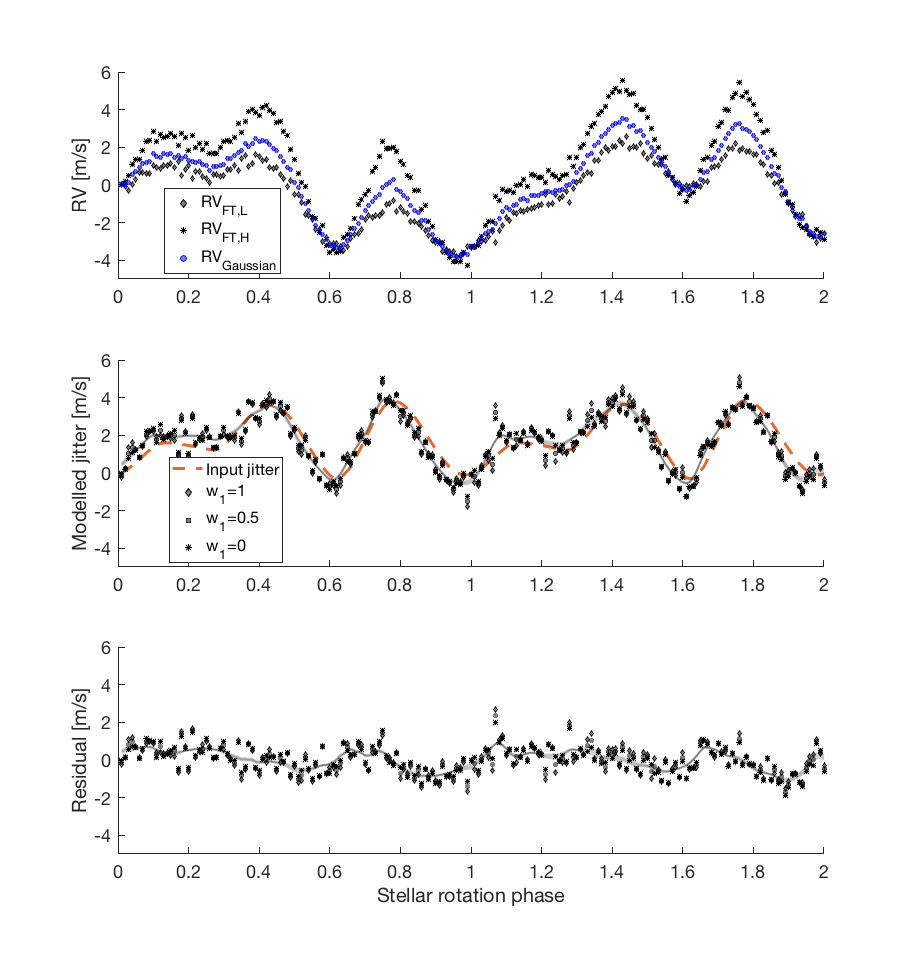
\includegraphics[width = 0.99 \linewidth]
{./Figures/Methods/5-PLANET_AND_JITTER2.png}
\caption[Jitter model]
{Construct jitter model from simulation data.}
\label{fig:PLANET_AND_JITTER}
\end{figure} 
%-------------
\FloatBarrier

%----------------------------------------------------------------------------------------
\subsection{Planetary radial velocity recovery}
Having obtained the jitter model (Eq.~\ref{eq:jitter_model_final}) and knowing $RV_\text{planet}$ follows a Keplerian orbital motion, we can turn our planetary radial velocity recovery into a model fitting problem, in which the parameters of the jitter model (such as the scaling factor) and that of the Keplerian orbit (such as amplitude, orbital period and phase) are to be determined. 

Alternatively, we can bypass the jitter model. Revisiting the Equations \ref{eq:RV_Gau}-\ref{eq:RV_FTH}, we rewrite them by observation number $i (i=1,2,\ldots,N)$ and switch the notations to obtain the following $3N$ independent linear equations:
\begin{align}
	X_i 		&= P_i + J_i				\label{eq:XX} \\
	Y_i 		&= P_i + k_y \cdot J_i	\label{eq:YY} \\
	Z_i 		&= P_i + k_z \cdot J_i 	\label{eq:ZZ}
\end{align}
where $X_i, Y_i$ and $Z_i$ replace the three measurable radial velocities $RV_\text{Gaussian}$, $RV_\text{FT,L}$ and $RV_\text{FT,H}$; $P_i$ and $J_i$ are the planetary radial velocities and the jitter; $k_y$ and $k_z$ are the scaling factors $k_L$ and $k_H$. Substituting $J_i = X_i - P_i$ from Eq.~\ref{eq:XX}, we can simply the system to the following $2N$ independent linear equations:
\begin{align}
	Y_i 		&= k_y \cdot X_i + (1-k_y)P_i	\label{eq:YYY} \\
	Z_i 		&= k_z \cdot X_i + (1-k_z)P_i	\label{eq:ZZZ}.
\end{align}
The number of unknowns is $(N+4)$, including $N$ from $P_i$, 2 from $k_y$ and $k_z$, and another 2 from the previously omitted constant offsets. Normally we have $N \gg 1$, so that the number of independent equations ($2N$) is larger than the number of degrees of freedom $(N+4)$ in the system, meaning the system can be uniquely solved by optimization, such as least square minimization of the objective function:
\begin{equation}
	\sum_{i=1}^{N} \Bigg[w_{y,i}\Big(k_y \cdot X_i + (1-k_y)P_i - Y_i \Big)^2 + w_{z,i}\Big(k_z \cdot X_i + (1-k_z)P_i- Z_i \Big)^2 \Bigg]
\label{eq:objective_function}
\end{equation}
where $w_{y,i}$ and $w_{z,i}$ are pre-determined parameters (e.g. determined by the sizes of errorbars of the observed radial velocities) used to weight the linear systems. In addition, this approach becomes identical to constructing a jitter model (Eq.~\ref{eq:jitter_model_final}) in cases that (1) $w_{y,i}=1, w_{z,i}=0 (i=1,2,\ldots,N)$ and $w_1=1, w_2=0$; (2) $w_{y,i}=0, w_{z,i}=1 (i=1,2,\ldots,N)$ and $w_1=0, w_2=1$. 

%----------------------------------------------------------------------------------------
\subsection{End-to-end simulations}

In this subsection we will be testing three categories of determining a planet candidate in the presence of jitter through end-to-end simulations:
\begin{enumerate}
	\item In a system where the amplitude of jitter is comparable to that of the planetary radial velocities, can we recover the planet orbital parameters better with our Fourier phase analysis than without jitter correction? 
	\item In a system where the planetary radial velocities dominate and jitter is negligible, does our method give at least equally good results as the traditional methods? 
	\item In a system where jitter is the only source of radial velocities, can our method inform us about it?
\end{enumerate}
We will also answer the important question: how to classify these three categories in the first place? 

The spectral line profile simulator setup is the same as previously, except setting S/N to be 2,000 to imitate a real-world cross-correlation function of a line profile from HARPS. The jitter amplitude is fixed at roughly 2~m/s, so we will adjust the planetary orbital amplitude to satisfy these three categories. We will run 200 trails, each trail with 60 randomly selected samples clustered in 12 groups, out of a total of 400 equally spaced samples from four stellar rotation periods. 

The tests are divided into two main groups for comparison:
\begin{enumerate}
	\item Fit $RV_\text{Gaussian}$ by Keplerian orbit alone;
	\item Fit $RV_\text{Gaussian}$ by Keplerian orbit with jitter model correction. The following three variations of model fitting have been tested:
   \begin{enumerate}
     \item Jitter model constructed with $RV_\text{Gaussian}$ and $RV_\text{FT,L}$ only, i.e. $w_1=1$ and $w_2=0$;
     \item Jitter model constructed with $RV_\text{Gaussian}$ and $RV_\text{FT,H}$ only, i.e. $w_1=0$ and $w_2=1$;
     \item Jitter model constructed with $RV_\text{Gaussian}$, $RV_\text{FT,L}$ and $RV_\text{FT,H}$. We test with $w_1=0.5$ and $w_2=0.5$;
   \end{enumerate}
\end{enumerate}
The parameters for the fitting is obtained by Markov chain Monte Carlo (MCMC) sampling. Each radial velocity data is equally weighted as they have the same S/N. We find that among the three variations of jitter correction treatments, the one left with the least rms statistically returns the best parameter fitting performance, so we will choose the one to represent the fitting from Group2. 

%----------------------------------------------------------------------------------------
\subsubsection{Stellar jitter as strong as planetary signal}

The injected planet has the same parameter settings as in \S\ref{sec:check}, i.e. circular orbit with amplitude $A = 2$~m/s,
orbital frequency ratio $\nu = \nu_\text{orb}/\nu_\text{rot}= 0.7$ and initial phase $\omega = 1$~rad. After running for 200 trails, we recover the parameters for each trail (Fig.~\ref{fig:Corner}) and obtain the histograms of the recovered orbital parameters, e.g. the amplitude and the orbital period (here the orbital frequency ratio) that we mostly concerned about (Fig.~\ref{fig:Histogram}). 

%-------------
\begin{figure}[tbp]	
    \begin{subfigure}[b]{0.49\textwidth}
        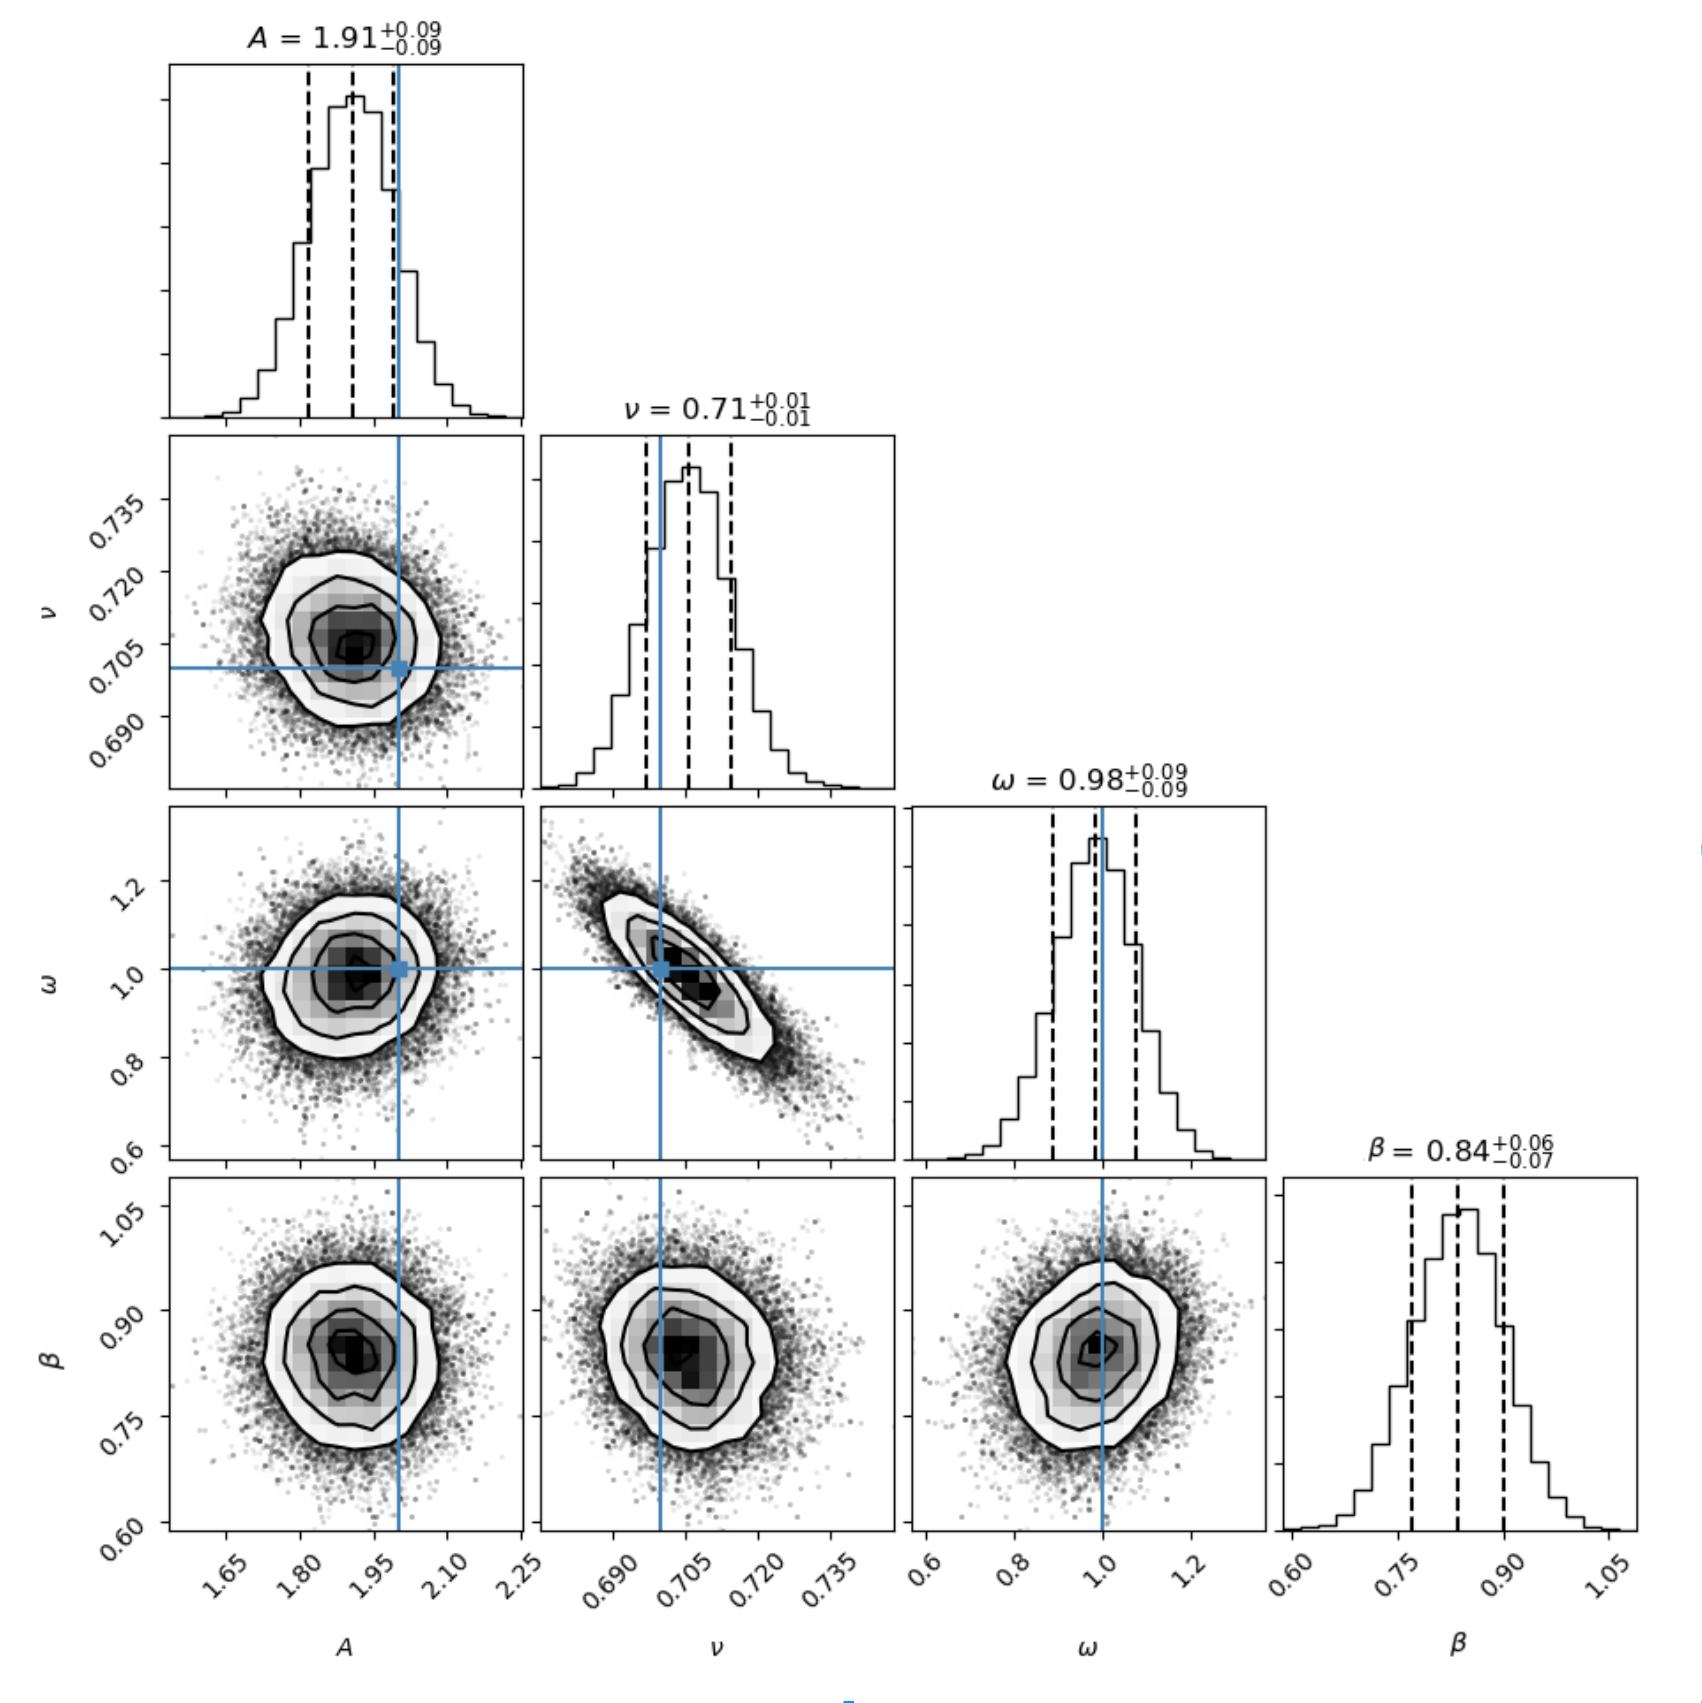
\includegraphics[width=\textwidth]{./Figures/Methods/Fitting_3-MCMC2.png}
        \caption{No jitter correction}
    \end{subfigure}
	~
    \begin{subfigure}[b]{0.49\textwidth}
        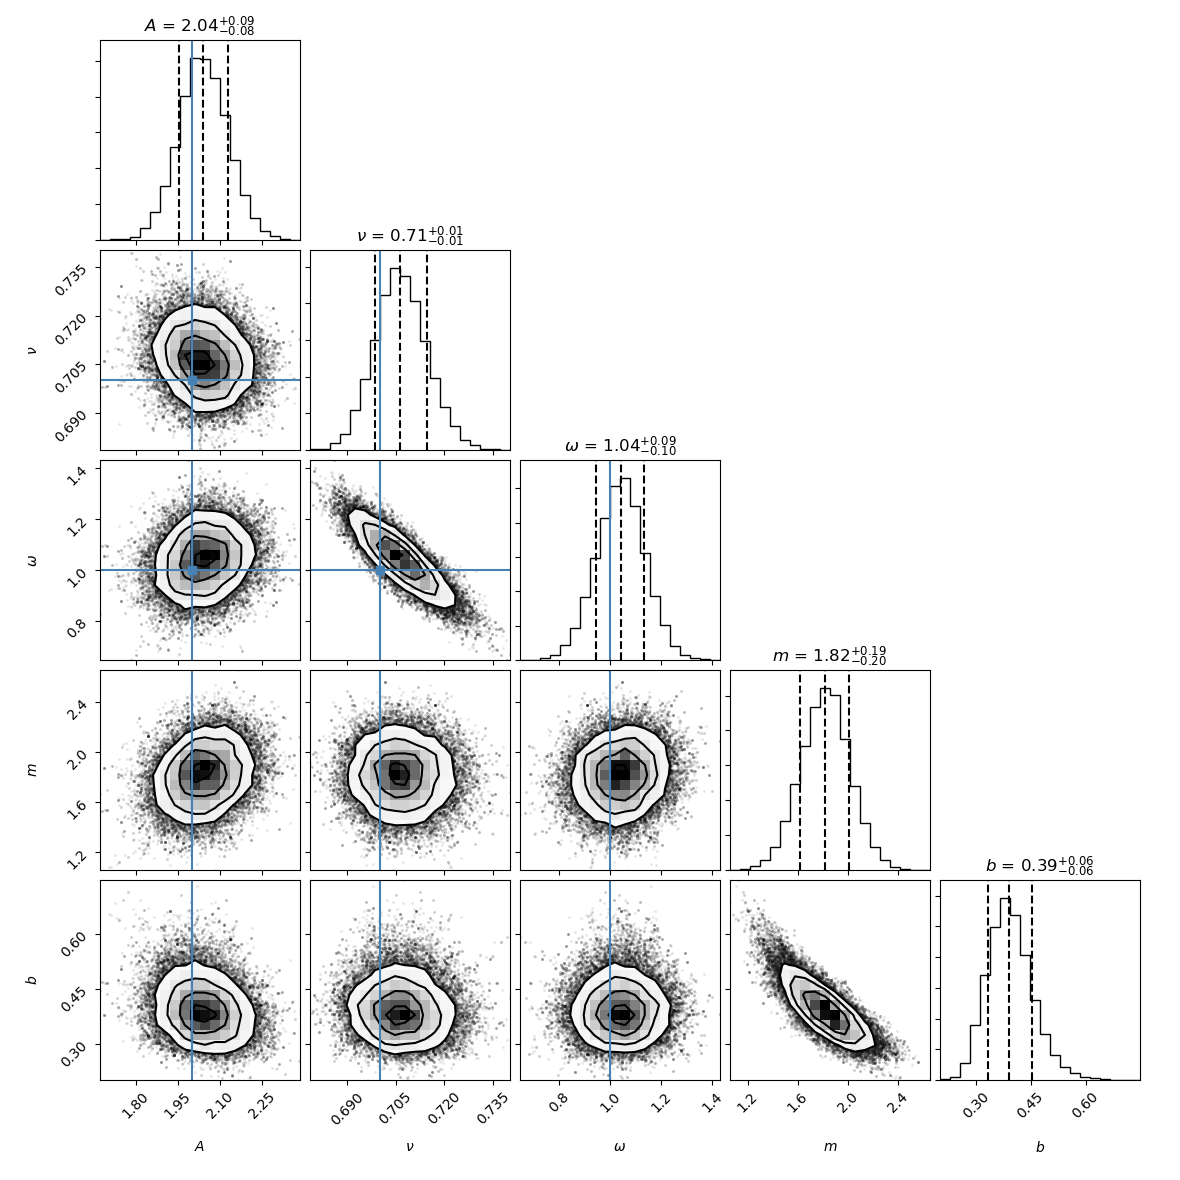
\includegraphics[width=\textwidth]{./Figures/Methods/Fitting_3-MCMC1_XY.png}
        \caption{Jitter correction applied}
    \end{subfigure}	
    \caption[Corner plots of MCMC]
    {Examples of two corner plots showing the successfully recovered planetary orbital parameter with MCMC sampling. The blue solid lines indicate the true values of the input orbital parameters. The three dashed lines of each histogram indicate the median and $1\sigma$ on both sides.}
\label{fig:Corner}
\end{figure}    
%-------------

%-------------
\begin{figure}[tbp]	
    \begin{subfigure}[b]{0.49\textwidth}
        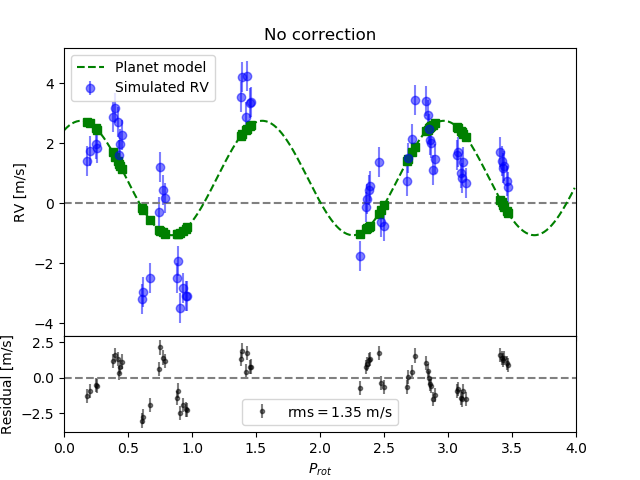
\includegraphics[width=\textwidth]{./Figures/Methods/Fitting_5-Fit2.png}
    \end{subfigure}
	~
    \begin{subfigure}[b]{0.49\textwidth}
        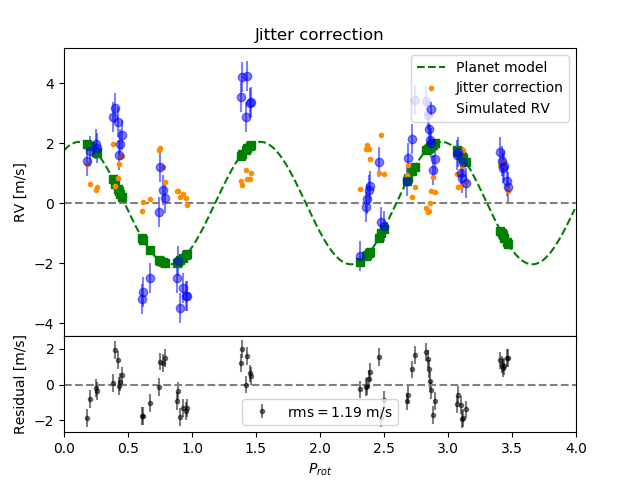
\includegraphics[width=\textwidth]{./Figures/Methods/Fitting_5-Fit1_XY.png}
    \end{subfigure}	
    \caption[Planet recovery ($A = 2$~m/s)]
    {Radial velocity fitting. Theses are two fittings that comes out from the MCMC corner plots in Fig.~\ref{fig:Corner} on the same set of simulated radial velocities. The discrepancy between the simulated radial velocities and the planet model is accounted for by the jitter model, and thus applying the jitter correction reduces the rms of the residual.}
\label{fig:Planet_recovery}
\end{figure}    
%-------------

%-------------
\begin{figure}[tbp]	
    \begin{subfigure}[b]{0.49\textwidth}
        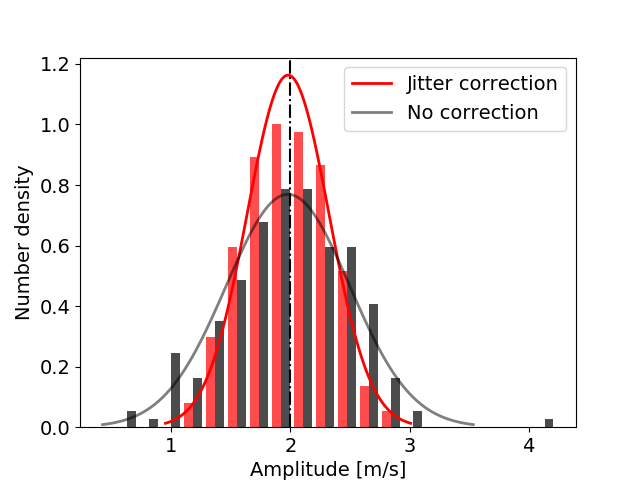
\includegraphics[width=\textwidth]{./Figures/Methods/Histogram_new1.png}
    \end{subfigure}
	~
    \begin{subfigure}[b]{0.49\textwidth}
        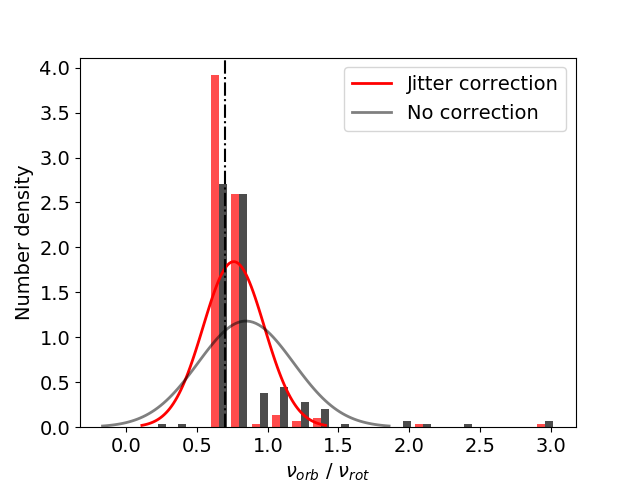
\includegraphics[width=\textwidth]{./Figures/Methods/Histogram_new2.png}
    \end{subfigure}	
    \caption[Histogram of recovered orbital parameters ($A = 2$~m/s)]
    {Histogram of recovered orbital parameters with a Gaussian profile fitted on top. The results from jitter correction are labelled in red (left in the histogram and dark in the Gaussian profile) and that without correction are labelled in grey (right in the histogram and light the Gaussian profile).}
\label{fig:Histogram}
\end{figure}    
%-------------

To quantitatively describe their performances, we calculate the percentage of parameters successfully recovered within 5\% and 10\% of the true values as summarized in Table~\ref{table:a=2}. For example, 15\% of the 200 trails have both the amplitude ($A$) and orbital frequency ($\nu_\text{orb}/\nu_\text{rot}$) successfully recovered within 5\% of the true parameters with jitter correction applied, while only 8\% of them achieve such a precision without jitter correction. 

%-------------
\begin{table}[h!]
\centering
\begin{tabular}{|c|c|c|c|c|}
\hline
\multirow{2}{*}{Percentage} 	& \multicolumn{2}{c|}{5\% limit}  & \multicolumn{2}{c|}{10\% limit}  \\ \cline{2-5} 
                  	& \multicolumn{1}{l|}{$\dagger$} & \multicolumn{1}{l|}{$\ddagger$} & \multicolumn{1}{l|}{$\dagger$} & \multicolumn{1}{l|}{$\ddagger$} \\ \hline
$A$  	 									& 16\% 		& 23\% 			& 32\% 			& 39\%             \\ \hline
$\nu_\text{orb}/\nu_\text{rot}$  			& 40\% 		& 58\%			& 67\%			& 89\%             \\ \hline
both $A$ and $\nu_\text{orb}/\nu_\text{rot}$ & 8\% 		& 15\%			& 23\%			& 37\%             \\ \hline
\end{tabular}
\caption{Proportion of recovered parameters within a 1\% or 5\% limit of $A = 2$~m/s and $\nu_\text{orb}/\nu_\text{rot} =0.7$. $\dagger$: no correction; $\ddagger$: jitter correction applied.}
\label{table:a=2}
\end{table}
%-------------
\FloatBarrier

%----------------------------------------------------------------------------------------

\subsubsection{Planetary signal dominates}

In this case, we set the orbital amplitude roughly 10 times as strong as the jitter, i.e. $A = 20$~m/s (Fig.~\ref{fig:Planet_recovery_a20}). This scenario hardly has impact on obtaining high precision of the orbital parameters of the planets using both approaches (Fig.~\ref{fig:Histogram20}), but applying jitter correction slightly improves the performance with an overall more precise measurements of the orbital parameters (Table.~\ref{table:a=20}). 

%-------------
\begin{figure}[htbp]	
    \begin{subfigure}[b]{0.49\textwidth}
        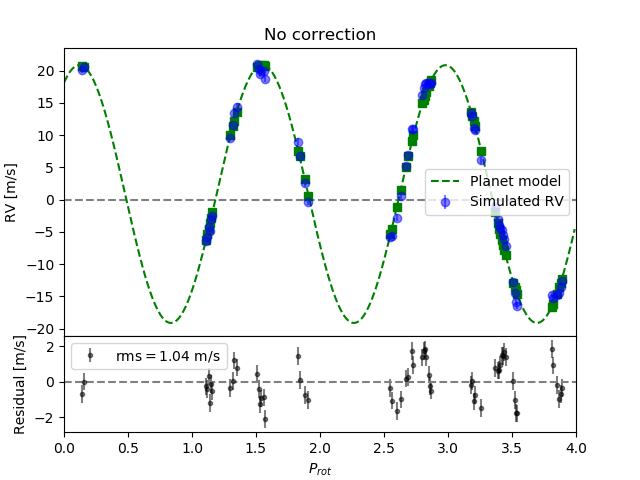
\includegraphics[width=\textwidth]{./Figures/Methods/Fitting_5-Fit2_a20.png}
    \end{subfigure}
	~
    \begin{subfigure}[b]{0.49\textwidth}
        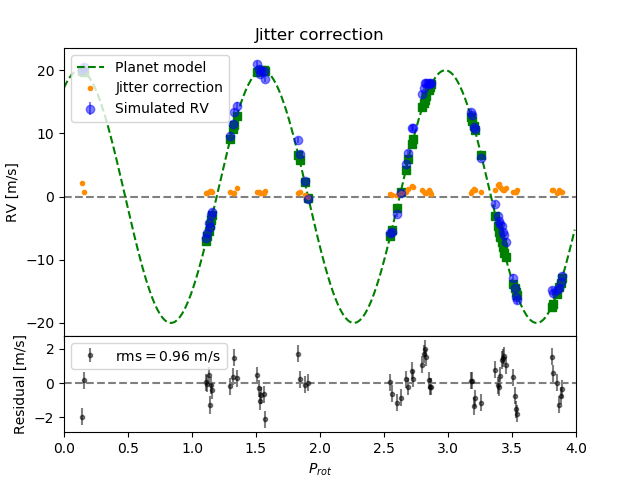
\includegraphics[width=\textwidth]{./Figures/Methods/Fitting_5-Fit1_XYZ_a20.png}
    \end{subfigure}	
    \caption[Planet recovery ($A = 20$~m/s)]
    {Same with Fig.~\ref{fig:Planet_recovery} except the input orbital amplitude of the planet being $A = 20$~m/s.}
\label{fig:Planet_recovery_a20}
\end{figure}    
%-------------

%-------------
\begin{figure}[htbp]	
    \begin{subfigure}[b]{0.49\textwidth}
        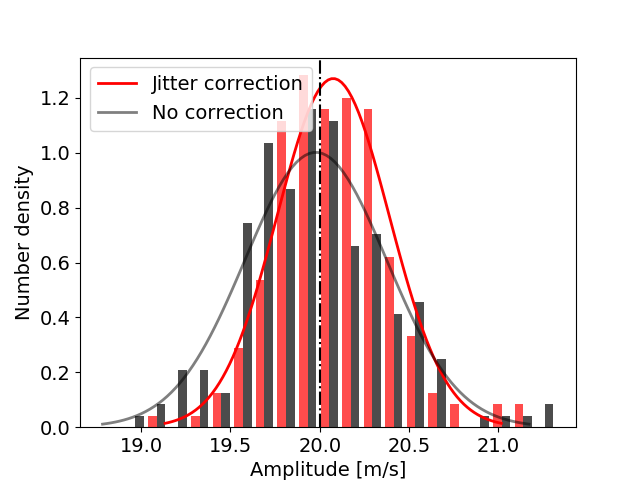
\includegraphics[width=\textwidth]{./Figures/Methods/Histogram_new1_a20.png}
    \end{subfigure}
	~
    \begin{subfigure}[b]{0.49\textwidth}
        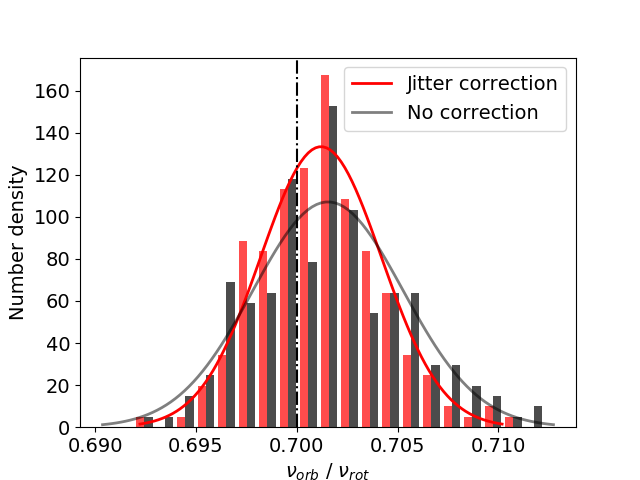
\includegraphics[width=\textwidth]{./Figures/Methods/Histogram_new2_a20.png}
    \end{subfigure}	
    \caption[Histogram of recovered orbital parameters ($A = 20$~m/s)]
    {Same with Fig.~\ref{fig:Histogram} except the input orbital amplitude of the planet being $A = 20$~m/s.}
\label{fig:Histogram20}
\end{figure}    
%-------------

%-------------
\begin{table}[h!]
\centering
\begin{tabular}{|c|c|c|c|c|}
\hline
\multirow{2}{*}{Percentage} 	& \multicolumn{2}{c|}{1\% limit}  & \multicolumn{2}{c|}{5\% limit}  \\ \cline{2-5} 
                  	& \multicolumn{1}{l|}{$\dagger$} & \multicolumn{1}{l|}{$\ddagger$} & \multicolumn{1}{l|}{$\dagger$} & \multicolumn{1}{l|}{$\ddagger$} \\ \hline
$A$  	 									& 41\% 		& 51\% 			& 98\% 			& 99\%             \\ \hline
$\nu_\text{orb}/\nu_\text{rot}$  			& 91\% 		& 97\%			& 100\%			& 100\%             \\ \hline
both $A$ and $\nu_\text{orb}/\nu_\text{rot}$ & 37\% 		& 49\%			& 98\%			& 99\%             \\ \hline
\end{tabular}
\caption{Proportion of recovered parameters within a 5\% or 10\% limit of $A = 20$~m/s and $\nu_\text{orb}/\nu_\text{rot} =0.7$. $\dagger$: no correction; $\ddagger$: jitter correction applied.}
\label{table:a=20}
\end{table}
%-------------
\FloatBarrier

\subsubsection{Stellar jitter only}

We set $A=0$~m/s so that the measured the radial velocity only comes from stellar variability. We implement the same approaches as above to see if the applying the jitter correction can return a null planet solution i.e. recovered amplitude smaller than the noise level.

The input jitter is the same as used in Fig.~\ref{fig:scaling_RV_FT}, showing the presence of three starspots in turns, mimicking the radial velocities of orbiting exoplanets. This is indeed the case in the histogram of ``recovered" orbital parameters (Fig.~\ref{fig:Histogram_null}): $\nu_\text{orb}/\nu_\text{rot}$ pops up at around 1, 2 and 3, with 3 being the most prominent. 

%-------------
\begin{figure}[htbp]	
    \begin{subfigure}[b]{0.49\textwidth}
        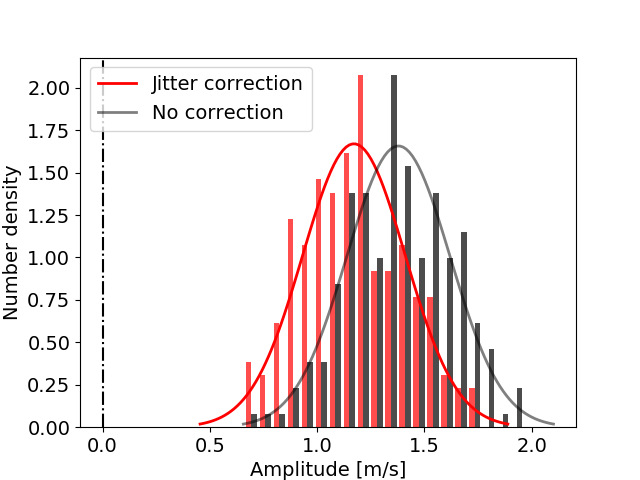
\includegraphics[width=\textwidth]{./Figures/Methods/Histogram_new1_null.png}
    \end{subfigure}
	~
    \begin{subfigure}[b]{0.49\textwidth}
        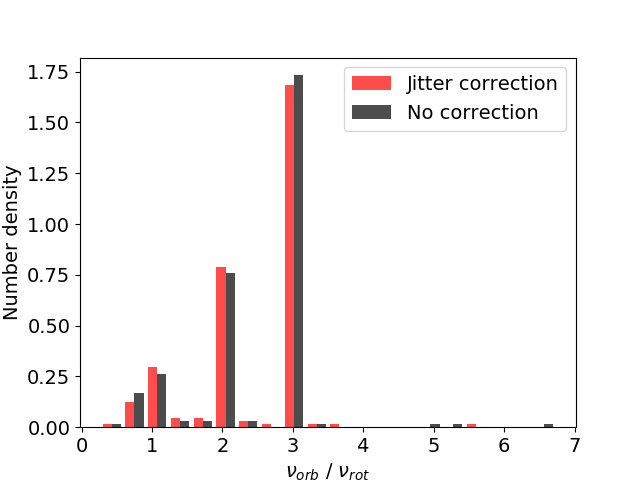
\includegraphics[width=\textwidth]{./Figures/Methods/Histogram_new2_null.png}
    \end{subfigure}	
    \caption[Histogram of recovered orbital parameters of null planets]
    {Histogram of ``recovered" orbital parameters of null planets.}
\label{fig:Histogram_null}
\end{figure}    
%-------------



%Unless we are sure of a null-planetary system where $RV_\text{planet} = 0$ and
%from Eq.~\ref{eq:RV_Gaussian} and Eq.~\ref{eq:RV_FT,L} we obtain
%\begin{equation}
%	k = RV_\text{jitter} / RV_\text{Gaussian},
%\end{equation} 
%normally $k$ cannot be directly calculated, so neither can $\alpha$ be.
%However, we could substitute the jitter model (Eq.~\ref{eq:jitter_model}) into Eq.~\ref{eq:RV_Gaussian}, such that
%\begin{equation}
%	RV_\text{Gaussian} = RV_\text{planet} + \alpha \cdot \Delta RV
%\label{eq:RV_fit}
%\end{equation}
%where $RV_\text{planet}$ is parametrised by Keplerian orbit(s) and both $RV_\text{Gaussian}$ and $\Delta RV$ 
%are measurable. 

%
%We will compare which group recovers the planet parameters better. 
%
%To better simulate the real observations, 40 data samples out of 200 from the two rotation periods are randomly selected.  
%
%It is defined if the input parameter lies within $1\sigma$ errorbar of the output parameter, it counts as a 
%successful detection. 
%
%For demonstration, we show one of the outputs in corner plots (Fig.~\ref{fig:Corner}) and the corresponding 
%radial velocity fitting (Fig.~\ref{fig:Planet_recovery}). The corner plot visually shows the how the walkers explore the parameter 
%space and their distribution. The histogram gives an example explaining how a ``successful detection" is qualified. 
%The radial velocity fitting plot demonstrates an example that implementing the jitter model effectively 
%accounts for the spurious signals in the raw radial velocity data, reducing the rms from 1.14~m/s to 0.55~m/s. 
%
%
%
%
%In the end, we run 100 trails for the end-to-end simulation. The random differences among these 100 trails come from:
%\begin{itemize}
%	\item photon noise given the S/N;
%	\item randomly selected 40 samplings in the 200 line profiles.
%\end{itemize}
%It turns out that in $46\%$ of the 100 trails are successful detections for both $A$ and $\nu$ when we 
%apply the jitter correction model, while this percentage is only $11\%$ without jitter correction. 
%In more detail, Fig shows that with jitter correction (in red), both of the amplitude and 
%orbital frequency ratio tend to be underestimated, which is shown opposite for the results without correction (in blue). 
%Moreover, the jitter corrected parameters are better constrained (i.e. with narrower distributions) and 
%performs much better in $\nu$ than without correction. While it is tempting to say the correct answer is more likely in between
%the results from these two fittings, we would need more tests to conclude. 



%----------------------------------------------------------------------------------------
\section{Fourier transform with real observations}
\label{\thesection}
\label{sec:observation}

\subsection{HD189733: Rossiter–McLaughlin effect as jitter}
\label{sec:HD189733}

HD189733 is a well studied binary star system. The main star HD189733~A is known to host a gas giant
exoplanet HD189733~b, first detected by transits (reference...) and later by Doppler spectroscopy (references...). 
It was also the first exoplanet transit observed in X-ray (references...). 

We choose this target for the following reasons:
\begin{itemize}
	\item The exoplanet is well confirmed;
	\item The host star is bright enough: $m_V=7.66$;
	\item The gas giant exoplanet causes a prominent apparent radial velocity while it transits ($\sim 40$~m/s)
	due to Rossiter–McLaughlin effect.
\end{itemize}

%-------------
\begin{figure}[tbp]
\centering
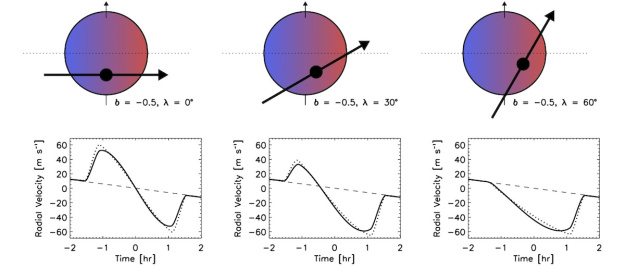
\includegraphics[width = 0.80 \linewidth]
{./Figures/Methods/rmeffect.jpg}
\caption[Demo: Rossiter–McLaughlin effect]
{Demo: Rossiter–McLaughlin effect (reference...). It is a apparent radial velocity
	change of the parent star due to an eclipsing binary (whether star or planet) that breaks the observed flux symmetry in the 
	stellar photosphere, resulting in imbalanced redshift and blueshift. It shows in this plot three different star-planet 
	alignments that causes three corresponding different shapes of radial velocity curve, and hence the radial velocity curve
	sheds information on the geometry of the alignment.}
\label{fig:rm-effect}
\end{figure} 
%-------------

We treat as if it were an ``active" star with one big dark starspot, as the Rossiter–McLaughlin effect 
causes the line profile deformed in a similar manner that a starspot would do (Fig.~\ref{fig:rm-effect}). 
We aim to test if our jitter model can account for the radial velocity variation from Rossiter–McLaughlin effect. 

The procedure is rather standardized. Both $RV_\text{Gaussian}$ and $RV_\text{FT}$ are calculated from the 
HARPS cross-correlation functions of the spectra. $\Delta RV = RV_\text{Gaussian} - RV_\text{FT}$ are then 
smoothed by a Gaussian filter. The prototype of the Rossiter–McLaughlin
radial velocity curve is already identifiable ($\Delta RV$ of the lower panel of Fig.~\ref{fig:HD189733}). 

%-------------
\begin{figure}[tbp]
\centering
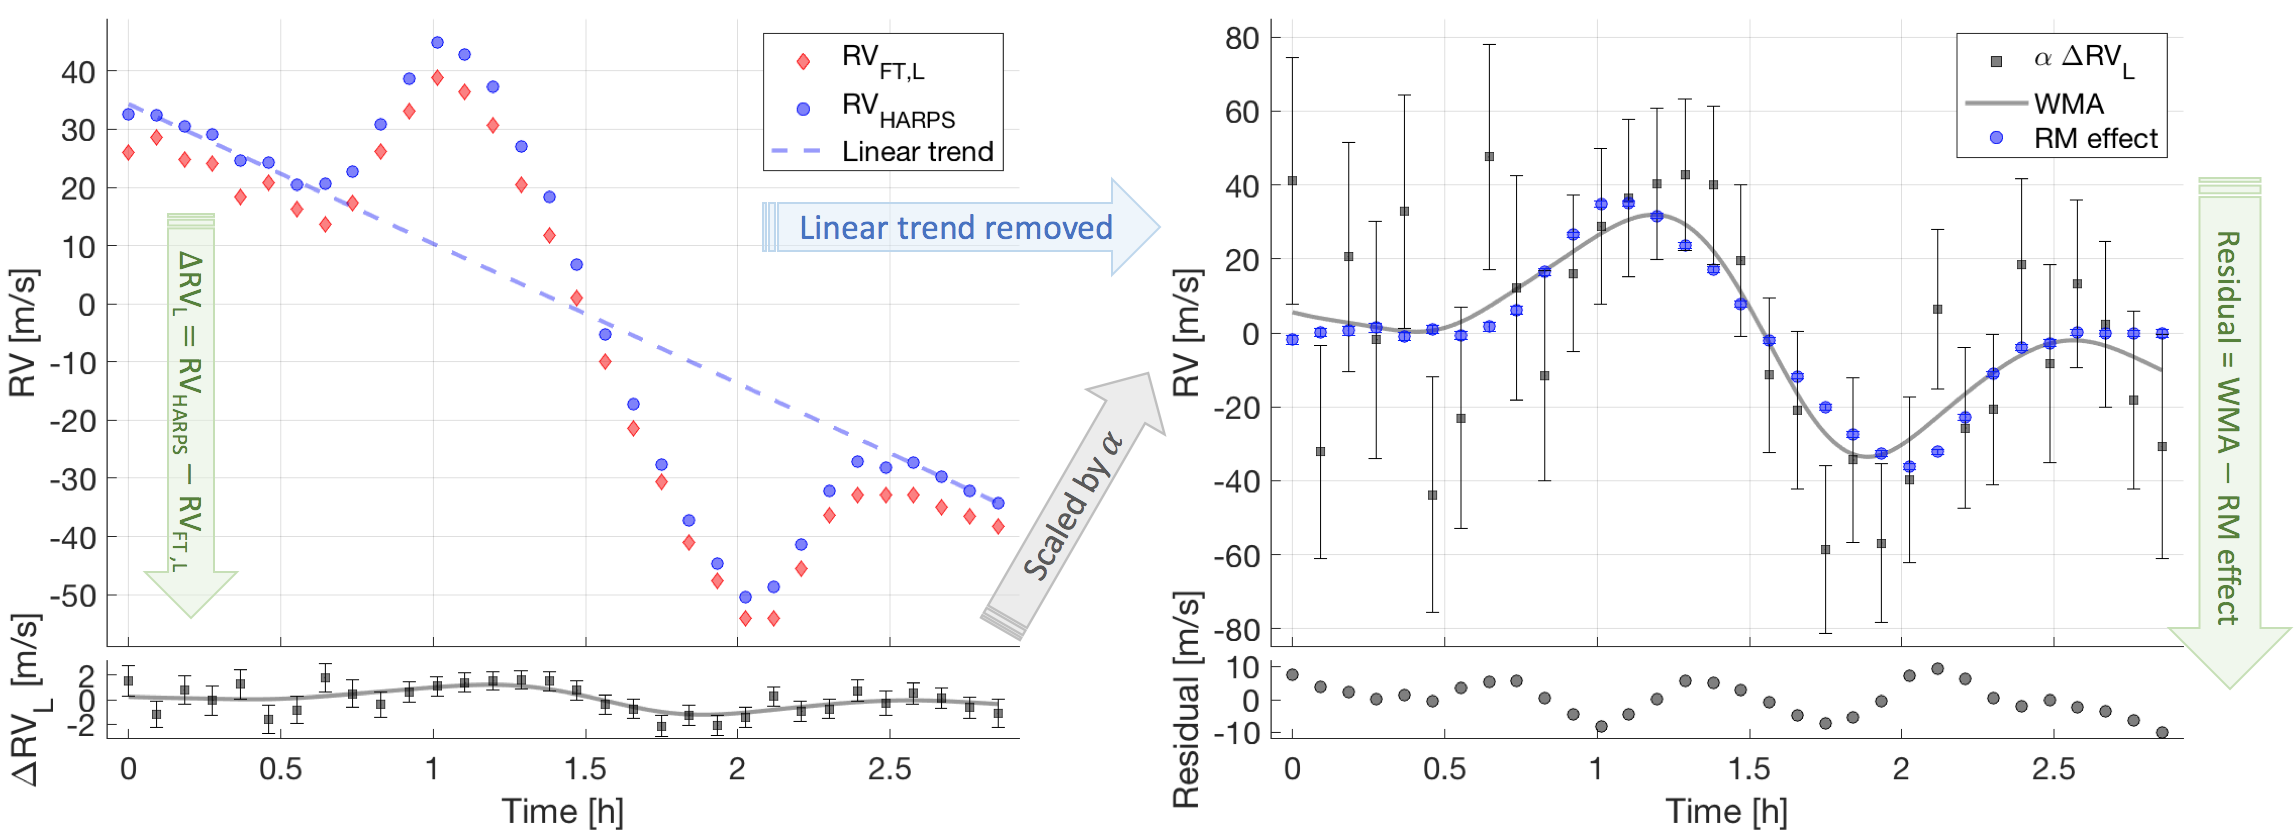
\includegraphics[width = 1.0 \linewidth]
{./Figures/Methods/HD189733.png}
\caption[HD189733: removal of Rossiter–McLaughlin effect as jitter]
		{HD189733: removal of Rossiter–McLaughlin effect as jitter. From $RV_\text{Gaussian}$ and $RV_\text{FT}$ to $\Delta RV$. The scattered $\Delta RV$ are smoothed by applying a moving average with a Gaussian filter and  further weighted according to the size of errorbar. It is then scaled by $\alpha$ to match the jitter (in this case the radial velocities of the observed Rossiter–McLaughlin effect). The residual is the difference between the smoothed jitter model and the observed Rossiter–McLaughlin effect. Errorbars are not plotted for the residuals for the reason that they will overwhelm the residual themselves.}
\label{fig:HD189733}
\end{figure} 
%-------------

During transit, as the parent star and the exoplanet are along the line of sight, there will be no contribution to radial velocity by the orbiting exoplanet. However, the radial velocity shows an inclined trend in this system. It is due to the other orbiting star in the binary star system. Considering the orbital period of the binary star estimated around 3,200 years (reference...), the radial velocity contribution from the other star during the timespan of transit ($\sim$ 0.08 days) can be treated linear. By removing such a linear trend, which is fitted for the non-transiting part, we can extract the observed Rossiter–McLaughlin radial velocity curve. It is treated as jitter and modelled by $\alpha \cdot \Delta RV$ (Fig.~\ref{fig:HD189733} upper right). Note that the errorbars of the jitter model also becomes a factor of $\alpha$ ($\alpha\gg 1$) larger; however, the model itself shows a descent approximation of the Rossiter–McLaughlin radial velocity curve. The difference between our modelled jitter and the observed Rossiter–McLaughlin effect peaks at $\sim 10$~m/s, a $\sim75\%$ removal of the jitter from $\sim 40$~m/s. 


\paragraph{Remarks}
The effective length of the smoothing kernel should be carefully chosen. In this case, it's chosen most effective within 
roughly one neighbouring data point on both size. While mitigating the effect of noise (especially for relatively lower
S/N data outside the transits), to which the Fourier transform is sensitive, it also smears the drastic velocity 
change when the planet ingresses and egresses the stellar disk. To solve this awkward situation, an adaptive 
(i.e. S/N dependent) effective length of the smoothing kernel may be used. 
%
%%-------------
%\begin{figure}[tbp]
%\centering
%\includegraphics[width = 0.80 \linewidth]
%{./Figures/Methods/9-RM_fit2.png}
%\caption[Rossiter–McLaughlin effect as jitter]
%{Rossiter–McLaughlin effect as jitter fitted with the jitter model.} 
%\label{fig:rm_as_jitter}
%\end{figure} 
%%-------------

\subsection{Examples 2}

HD\,49933 is an F2 main sequence star with an apparent magnitude of $m_V=5.8$ (\cite{Malaroda1975}), 

\subsection{Example 3}



\FloatBarrier
A float barrier will stop figures from going beyond this point. They are handy to make sure they don't go into the next section.

%----------------------------------------------------------------------------------------
%\clearpage
\section{References}
\label{\thesection}
\vspace{-1.5cm}
\setstretch{1.0}
\bibliographystyle{unsrt}
\bibliography{Bibliography}
\setstretch{1.3}
